\documentclass[11pt]{beamer}

\usetheme{Warsaw}
%\addtobeamertemplate{navigation symbols}{}{%
%    \usebeamerfont{footline}%
%    \usebeamercolor[fg]{footline}%
%    \hspace{1em}%
%    \insertframenumber/\inserttotalframenumber
%}

\beamertemplatenavigationsymbolsempty

\setbeamertemplate{footline}
{
  \leavevmode%
  \hbox{%
  \begin{beamercolorbox}[wd=.333333\paperwidth,ht=2.25ex,dp=1ex,center]{author in head/foot}%
    \usebeamerfont{author in head/foot} \hyperlink{Patrolling games}{\inserttitle}
  \end{beamercolorbox}%
  \begin{beamercolorbox}[wd=.333333\paperwidth,ht=2.25ex,dp=1ex,center]{title in head/foot}%
    \usebeamerfont{title in head/foot}\insertauthor
  \end{beamercolorbox}%
  \begin{beamercolorbox}[wd=.333333\paperwidth,ht=2.25ex,dp=1ex,right]{date in head/foot}%
    \usebeamerfont{date in head/foot}\insertshortdate{}\hspace*{2em}
    \insertframenumber{} / \inserttotalframenumber\hspace*{2ex} 
  \end{beamercolorbox}}%
  \vskip0pt%
}
\setbeamertemplate{headline}{}
\usefonttheme[onlymath]{serif}

\usepackage{color}
\usepackage{xcolor}
\usepackage{tikz}
\usepackage{amsmath}
\usepackage{amssymb}
\usepackage{amsthm}
\usepackage{amsfonts}
\usepackage{graphicx}
\usepackage{mathtools}
\usepackage{wrapfig}
\usepackage{multirow}
\usepackage{comment}
\usepackage{natbib}
\usepackage{appendix}
\usepackage[utf8]{inputenc}
%\usepackage{floatrow}
%\usepackage{newfloat}
\usepackage{subcaption}
\usepackage{bm}
\usepackage{hyperref}
\usepackage{tcolorbox}

\usetikzlibrary{calc}
\usetikzlibrary{fit}
\usetikzlibrary{shapes.misc,calc, positioning, hobby, backgrounds}

\tikzset{cross/.style={cross out, draw=black, minimum size=2*(#1-\pgflinewidth), inner sep=0pt, outer sep=0pt},
%default radius will be 1pt. 
cross/.default={1pt}}


%\DeclarePairedDelimiter{\floor}{\lfloor}{\rightfloor}
%\DeclarePairedDelimiter{\ceil}{\lceil}{\rceil}

\newcommand{\halflength}{\ensuremath{\floor{\frac{m}{2}}}}
\newcommand{\floor}[1]{\left \lfloor #1 \right \rfloor}
\newcommand{\ceil}[1]{\left \lceil #1 \right \rceil}
\newcommand{\pospart}[1]{\left( #1 \right)_{+}}
\newcommand{\negpart}[1]{\left( #1 \right)_{-}}
\newcommand{\set}[2]{\left\{ #1 \, | \, #2 \right\}}

\newcommand{\oneline}[1]{\resizebox{\dimexpr\paperwidth - 3ex}{!}{#1}}

%Text box tight style
\tcbset{mytight/.style={hbox,left=1mm,right=1mm,top=1mm,bottom=1mm,nobeforeafter}}

%\DeclareFloatingEnvironment[fileext=los,
 %   listname={List of Example Figures},
  %  name=Example Figure,
   % placement=tbhp,
    %within=section,]{examplefigure}

\author{Thomas Lowbridge}
\title{Patrolling games on graphs}
%\setbeamercovered{transparent} 
%\setbeamertemplate{navigation symbols}{} 
%\logo{} 
\institute{University Of Nottingham} 
\date{December 13, 2017} 
%\subject{} 
\begin{document}

\hypertarget{Patrolling games}{}
\begin{frame}
\titlepage
\end{frame}

%\begin{frame}
%\tableofcontents
%\end{frame}

\begin{frame}{Outline}

\begin{itemize}
\item Literature review
 \begin{itemize}
 \item Introduction to Game
  \begin{itemize}
  \item \hyperlink{Introduction to game: Pure game}{Pure game}
  \item \hyperlink{Introduction to game: Mixed game}{Mixed game}
  \end{itemize}
 \item Solved Graphs
  \begin{itemize}
  \item \hyperlink{Solved graphs: Hamiltonian graphs}{Hamiltonian graphs}
  %\item \hyperlink{Solved graphs: Complete bipartite graphs}{Complete bipartite graph}
  %\item \hyperlink{Solved graphs: Star graph}{Star graph}
  \item \hyperlink{Solved graphs: Line graph}{Line graph}
  \end{itemize}   
 \end{itemize}
\item \hyperlink{Problem with diametric strategy}{Problem with line graph strategy}
\item \hyperlink{Correction of diametric line graph strategy}{Correction of line graph strategy}
\item \hyperlink{Extension of correction strategy}{Extension of correction strategy}
%\item \hyperlink{Introduction to the elongated star}{Introduction to the elongated star}
\item \hyperlink{Future work}{Future work}
\end{itemize}
\end{frame}

\section[]{Pure game}
\hypertarget{Introduction to game: Pure game}{}
\begin{frame}{\insertsection}

A Patrolling game, \textcolor{purple}{$G=G(Q,T,m)$} is made of 3 major components
\begin{itemize}
\item A \textcolor{purple}{Graph, $Q=(N,E)$}, made of nodes, $N$ ($|N|=n$), and a set of edges, $E$.
\item A \textcolor{purple}{time horizon parameter, $T$} (with set $\mathcal{T}=\{0,1,...,T-1\}$).
\item An \textcolor{purple}{attack length parameter, $m$}.
\end{itemize}

\pause

The game involves two players, the patroller and the attacker.
\begin{itemize}
\item The \textcolor{blue}{patroller's strategy} is a walk (with waiting) on the graph, \textcolor{blue}{$W:\mathcal{T} \rightarrow  N$}.
\item The \textcolor{red}{attacker's strategy} is a node, \textcolor{red}{$i$} and starting time, \textcolor{red}{$\tau$}.
\end{itemize} 
The strategies are collected into the sets, $\mathcal{W}$ and $\mathcal{A}$ , for the patroller and attacker respectively, with some arbitrary labelling inside the set to form strategies $W_{i}$ and $A_{j}$.

\end{frame}

\begin{frame}{Payoff}
The game is formulated as \textcolor{purple}{win-lose} (a zero-sum) game with a payoff for the patroller of
\begin{align*}
P(W,(i,\tau))=\left\{ \begin{array}{l}
1 \text{  if  } i \in \left\{ W(\tau),W(\tau+1),...,W(\tau+m-1) \right\} ,\\
0 \text{  if  } i \notin \left\{ W(\tau),W(\tau+1),...,W(\tau+m-1) \right\} .\\
\end{array}\right.
\end{align*}
With a pure payoff matrix $\mathcal{P}=(P(W_{i},A_{j}))_{i \in \{ 1,...,|\mathcal{W}| \}, j \in \{ 1,...,|\mathcal{A}| \}}$


\textbf{Note.} The attackers payoff is simply negative the patroller payoff.
\end{frame}


\begin{frame}{Example of a pure game}
The game played on $Q$ as below with $m=3$ and $T=7$

\begin{center}
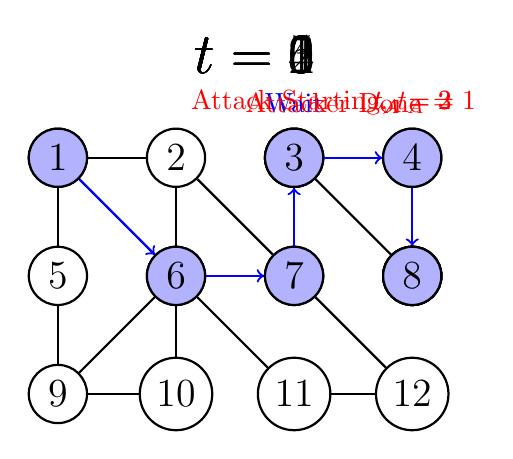
\begin{tikzpicture}[-,auto,node distance=1.5cm,
                    thick,main node/.style={circle,fill=white,draw,font=\sffamily\Large\bfseries}]

  \node[main node] (1) {$1$};
  \node[main node] (2) [right of=1] {$2$};
  \node[main node] (3) [right of=2]  {$3$};
  \node[main node] (4) [right of=3]  {$4$};
  \node[main node] (5) [below of=1]  {$5$};
  \node[main node] (6) [below of=2]  {$6$};
  \node[main node] (7) [below of=3]  {$7$};
  \node[main node] (8) [below of=4]  {$8$};
  \node[main node] (9) [below of=5]  {$9$};
  \node[main node] (10) [below of=6]  {$10$};
  \node[main node] (11) [below of=7] {$11$};
  \node[main node] (12) [below of=8] {$12$}; 

  \path[every node/.style={font=\sffamily}]
    (1) edge (2)
    (1) edge (5)
    (1) edge (6)
    (2) edge (6)
    (2) edge (7)
    (3) edge (7)
    (3) edge (4)
    (3) edge (8)
    (4) edge (8)
    (5) edge (9)
    (6) edge (7)
    (6) edge (10)
    (6) edge (11)
    (6) edge (9)
    (7) edge (12)
    (9) edge (10)
    (11) edge (12)
    ;

 %\node (GraphLabel) [shift={(0,1)}] at (1) {$Q$}; 

%Slide 2 (first animation)
  \visible<2>{
  \node (TimeLabel) [shift={(2.5,1.3)}] at (1) {\huge $t=0$};
  \node[main node,fill=blue!30] (1) at (1) {$1$};
  \path[->,color=blue] (1) edge (6); 
    }
%Slide 3
  \visible<3>{
   \node (TimeLabel) [shift={(2.5,1.3)}] at (1) {\huge $t=1$};
  \node[main node,fill=blue!30] (6) at (6) {$6$};
  \path[->,color=blue] (6) edge (7); 
    }
%Slide 4
  \visible<4>{
   \node (TimeLabel) [shift={(2.5,1.3)}] at (1) {\huge $t=2$};
  \node[main node,fill=blue!30] (7) at (7) {$7$};
  \path[->,color=blue] (7) edge (3);
  
  \node[main node,fill=red!30] (8) at (8) {$8$};
  \node[color=red] (Attacktimelabel) [shift={(-1,2.2)}] at (8) {Attack Starting, $t_{A}=1$};
    }
%Slide 5
  \visible<5>{
   \node (TimeLabel) [shift={(2.5,1.3)}] at (1) {\huge $t=3$};
  \node[main node,fill=blue!30] (3) at (3) {$3$};
  \node[color=blue] (WaitingLabel) [shift={(0,0.7)}] at (3) {Wait};
  
  \node[main node,fill=red!30] (8) at (8) {$8$};
  \node[color=red] (Attacktimelabel) [shift={(0,2.2)}] at (8) {$t_{A}=2$}; 
    }
%Slide 6
  \visible<6>{
   \node (TimeLabel) [shift={(2.5,1.3)}] at (1) {\huge $t=4$};
  \node[main node,fill=blue!30] (3) at (3) {$3$};
  \path[->,color=blue] (3) edge (4);
  
  \node[main node,fill=red!30] (8) at (8) {$8$};  
  \node[color=red] (Attacktimelabel) [shift={(0,2.2)}] at (8) {$t_{A}=3$};
    }
%Slide 7
  \visible<7>{
   \node (TimeLabel) [shift={(2.5,1.3)}] at (1) {\huge $t=5$};
  \node[main node,fill=blue!30] (4) at (4) {$4$};
  \path[->,color=blue] (4) edge (8); 
  
  \node[color=red] (Attacktimelabel) [shift={(-1,2.2)}] at (8) {Attacker Done};
    }    
%Slide 8
  \visible<8>{
   \node (TimeLabel) [shift={(2.5,1.3)}] at (1) {\huge $t=6$};
  \node[main node,fill=blue!30] (8) at (8) {$8$}; 
    }                 
\end{tikzpicture}

\end{center}
\only<1>{
\begin{itemize}
\item[] \textcolor{blue}{Patroller:} \textcolor{blue}{ $W(0)=1$ , $W(1)=6$ , $W(2)= 7$ , $W(3)=3$ , $W(4)=3$ , $W(5)=4$ , $W(8)= 8$}
\item[] \textcolor{red}{Attacker:} \textcolor{red}{$(8,2)$}
\end{itemize}
}
\only<8>
{
The attacker fails to catch the patroller, therefore the patroller loses (and the attacker wins) meaning a payoff of $0$ for the patroller (and $-1$ for the attacker).
}
\end{frame}

\section[]{Introduction to game: Mixed game}
\hypertarget{Introduction to game: Mixed game}{}
\begin{frame}{Mixed game formulation}
Both the patroller and attacker will play their pure strategies with certain probabilities, let \textcolor{blue}{$\bm{\pi}$} be a mixed strategy for the patroller and let \textcolor{red}{$\bm{\phi}$} be a mixed strategy for the attacker. We collect these into the sets $\Pi$ and $\Phi$ for the patroller and attacker respectively.

\pause

Then the payoff for the patroller of this mixed game becomes
\begin{align*}
P(\bm{\pi} ,\bm{\phi})=\sum\limits_{i=1}^{|\mathcal{W}|} \sum\limits_{j=1}^{|\mathcal{I}|} \mathcal{P}_{i,j} \bm{\pi} _{i} \bm{\phi}_{j}
=\bm{\pi} \mathcal{P} \bm{\phi}
\end{align*}

By using the pure payoff as $1$ when capture occurs and $0$ otherwise, the \textcolor{purple}{mixed payoff is equivalent to the probability of capture}.

\pause

By standard game theory results, we define the value of the game to be
\textcolor{purple}{$$V(G) \equiv \max\limits_{\bm{\pi} \in \Pi} \min\limits_{\bm{\phi} \in \Phi} P(\bm{\pi},\bm{\phi})=\min\limits_{\bm{\phi} \in \Phi} \max\limits_{\bm{\pi} \in \Pi} P(\bm{\pi},\bm{\phi})$$}
and we will seek its value by getting upper and lower bounds.
\end{frame}

%\begin{frame}{Nash equilibria and optimal solutions}
%\begin{definition}[Mixed Nash equilibrium]
%A choice of $\bm{\pi}^*$ and $\bm{\phi}^*$ is said to be in \textit{Nash equilibrium} if 
%\begin{align*}
%P(\bm{\pi}^*,\bm{\phi}^*) \geq P(\bm{\pi},\bm{\phi}^*) \quad \forall \bm{\pi} \in \Pi , \\
%P(\bm{\pi}^*,\bm{\phi}^*) \geq P(\bm{\pi}^*,\bm{\phi}) \quad \forall \bm{\phi} \in \Phi .
%\end{align*}
%\end{definition}
%
%\pause
%
%\begin{definition}[Optimal solution]
%let $N$ be the set of all Nash equilibria then we say that $(\bm{\pi}^{*},\bm{\phi}^{*}) \in N$ is an \textit{optimal solution} if
%$$P(\bm{\pi}^{*},\bm{\phi}^{*}) \geq P(n) \quad \forall n \in N$$ 
%\end{definition}
%
%\textbf{Note.} It is possible that no optimal solution exists
%
%\pause
%
%Luckily in zero-sum games are guaranteed to to have at least one optimal solution and any nash-equilbrium is optimal.
%
%\end{frame}
%
%\begin{frame}{Game Value}
%
%\begin{theorem}[Minimax Theorem (John Neumann, 1928)]
%Let $X \subset \mathbb{R}^{n}$ and $Y \subset \mathbb{R}^{m}$ be compact convex sets and let $f: X \times Y \rightarrow \mathbb{R}$ be a continuous convex-concave function then
%$$\min\limits_{x \in X} \max\limits_{y \in Y} f(x,y) = \max\limits_{y \in Y} \min\limits_{x \in X} f(x,y) $$
%\end{theorem}
%
%\textbf{Note.} Convex-concave means convex for a fixed $y$ and concave for a fixed $x$.
%
%\pause
%Now $\Pi$ and $\Phi$ are both compact convex sets and as our game is zero-sum our payoff function $P(\bm{\pi},\bm{\phi})$ is convex-concave. Solving the minimax problem is equivalent to Nash-equilibrium and are hence optimal solutions.
%
%
%This gives rise to the game's value, as given by \textcolor{purple}{$$V(G) \equiv \max\limits_{\bm{\pi} \in \Pi} \min\limits_{\bm{\phi} \in \Phi} P(\bm{\pi},\bm{\phi})=\min\limits_{\bm{\phi} \in \Phi} \max\limits_{\bm{\pi} \in \Pi} P(\bm{\pi},\bm{\phi})$$}
%In the patrolling game this is found by getting upper and lower bounds on the value.
%\end{frame}

\section[]{Solved graphs: Hamiltonian graphs}
\hypertarget{Solved graphs: Hamiltonian graphs}{}
\begin{frame}{\insertsection}

A graph is Hamiltonian if it is possible to find a \textcolor{purple}{cycle which visits every node exactly once} (apart from the start/finish).

\begin{block}{Hamiltonian graphs}
A Hamiltonian graph has the value $V=\frac{m}{n}$
\end{block}


Two common Hamiltonian graphs are the Cyclic graph (of n nodes $C_{n}$) and the Complete graph (of n nodes $K_{n}$).
\begin{center}
\begin{figure}

\begin{tabular}{@{}c@{}}
  \begin{tabular}{c}
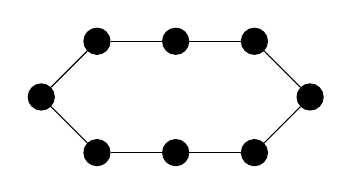
\begin{tikzpicture}[baseline=(current bounding box.north),-,auto,node distance=1cm,
                    main node/.style={circle,draw,fill=black,font=\sffamily\bfseries}]

  \node[main node] (1) {};
  \node[main node] (2) [above right of=1] {};
  \node[main node] (3) [right of=2] {};
  \node[main node] (4) [right of=3] {};
  \node[main node] (5) [below right of=4] {};
  \node[main node] (6) [below left of=5] {};
  \node[main node] (7) [left of=6] {};
  \node[main node] (8) [left of=7] {};
  

  \path[every node/.style={font=\sffamily}]
  (1) edge (2)
  (2) edge (3)
  (3) edge (4)
  (4) edge (5)
  (5) edge (6)
  (6) edge (7)
  (7) edge (8)
  (8) edge (1);

   
\end{tikzpicture}
     
      \\ \small $C_{8}$
  \end{tabular} \qquad
  \begin{tabular}{c}
  
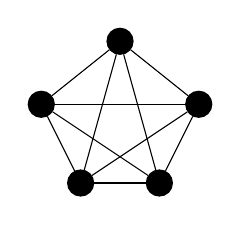
\begin{tikzpicture}[baseline=(current bounding box.north),-,auto,node distance=1cm,
                    main node/.style={circle,draw,fill=black,font=\sffamily\bfseries}]

  \node[main node] (1) {};
  \node[main node] (2) [shift={(1,-0.8)}] at (1) {};
  \node[main node] (3) [shift={(0.5,-1.8)}] at (1) {};
  \node[main node] (4) [shift={(-0.5,-1.8)}] at (1) {};
  \node[main node] (5) [shift={(-1,-0.8)}] at (1) {};

  

  \path[every node/.style={font=\sffamily}]
  (1) edge (2)
      edge (3)
      edge (4)
      edge (5)
  (2) edge (3)
      edge (4)
      edge (5)    
  (3) edge (4)
      edge (5)
  (4) edge (5);


   
\end{tikzpicture}

 \\ \small $K_{5}$
  \end{tabular} \\
\end{tabular}
\caption{Examples of Cyclic and Complete graphs}
\end{figure}
\end{center}



\end{frame}

%\section[]{Solved graphs: Complete bipartite graphs}
%\hypertarget{Solved graphs: Complete bipartite graphs}{}
%\begin{frame}{\insertsection}
%
%A bipartite graph is a graph made of two non-adjacent sets, the complete version has all connections.
%
%\begin{block}{Complete bipartite graph}
%A complete bipartite graph, $K_{a,b}$ has the value
%$V=\frac{m}{2 \max (a,b)}$
%\end{block}
%
%\begin{center}
%\begin{figure}
%\begin{tabular}{c}
%\begin{tikzpicture}[baseline=(current bounding box.north),-,auto,node distance=1cm,
%                    main node/.style={circle,draw,fill=black,font=\sffamily\bfseries}]
%
%  \node[main node] (1) {};
%  \node[main node] (2) [below of=1] {};
%  \node[main node] (3) [below of=2] {};
%  \node[main node] (4) [right of=1] {};
%  \node[main node] (5) [below of=4] {};
%
%  
%
%  \path[every node/.style={font=\sffamily}]
%  (1) edge (4)
%      edge (5)
%  (2) edge (4)
%      edge (5)    
%  (3) edge (4)
%      edge (5);
%
%   
%\end{tikzpicture}
%\\ \small $K_{3,2}$
%\end{tabular}
%\caption{Example of a complete bipartite graph}
%\end{figure}
%
%\end{center}
%
%\end{frame}
%
%\section[]{Solved graphs: Star graph}
%\hypertarget{Solved graphs: Star graph}{}
%\begin{frame}{\insertsection}
%
%The star graph, $S_{n}$, is $n$ nodes adjacent only to the centre. 
%
%\begin{block}{Star graph}
%The star $S_{n} \equiv K_{1,n}$ so has the value $V=\frac{m}{2n}$
%\end{block}
%
%\begin{center}
%\begin{figure}
%\begin{tabular}{c}
%\begin{tikzpicture}[baseline=(current bounding box.north),-,auto,node distance=1cm,
%                    main node/.style={circle,draw,fill=black,font=\sffamily\bfseries}]
%
%  \node[main node] (1) {};
%  \node[main node] (2) [above of=1] {};
%  \node[main node] (3) [right of=1] {};
%  \node[main node] (4) [below of=1] {};
%  \node[main node] (5) [left of=1] {};
%
%  
%
%  \path[every node/.style={font=\sffamily}]
%  (1) edge (2)
%      edge (3)
%      edge (4)
%      edge (5);
%
%   
%\end{tikzpicture}
%\\ \small $S_{4}$
%\end{tabular}
%\caption{Example of a star graph}
%\end{figure}
%
%\end{center}
%
%\end{frame}
%
%\section[]{Solved graphs: Line graph}
%\hypertarget{Solved graphs: Line graph}{}
%\begin{frame}{\insertsection}
%
%The line graph, $L_{n}$, made of $n$ nodes each adjacent to two other nodes (apart from the ends)
%
%\begin{block}{Line graph}
%The line graph, $L_{n}$ has a value dependent on $(n,m)$
%\begin{enumerate}
%\item If $m > 2(n-1)$ then $V=1$.
%\item If $n-1 < m \leq 2(n-1)$ then $V=\frac{m}{2(n-1)}$
%\item If $m=2 , n\geq 3$ then $V=\frac{1}{\ceil{\frac{n}{2}}}$
%\item If $m=n-1 \text{ or } m=n-2  \text{ and } m=2k \text{ for some } k \geq 2 $ then $V=\frac{1}{2}$
%\item If $3 \leq m \leq n-3$ or  $m=n-2$ and $m=2k+1$ for some  $k \geq 1$ then $V=\frac{m}{m+n-1}$
%\end{enumerate}
%\end{block}
%\textbf{Note.} The solution for $m=1$ is known for every graph as $V=\frac{1}{|N|}=\frac{1}{n}$, and on a line graph if $m=n=2$ then we know $V=1$.
%\end{frame}

\begin{frame}{Line graph example}

\begin{center}
\begin{figure}
\begin{tabular}{c}
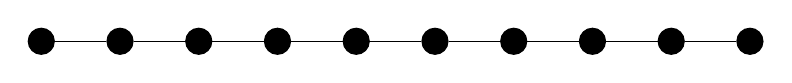
\begin{tikzpicture}[baseline=(current bounding box.north),-,auto,node distance=1cm,
                    main node/.style={circle,draw,fill=black,font=\sffamily\bfseries}]

  \node[main node] (1) {};
  \node[main node] (2) [right of=1] {};
  \node[main node] (3) [right of=2] {};
  \node[main node] (4) [right of=3] {};
  \node[main node] (5) [right of=4] {};
  \node[main node] (6) [right of=5] {};
  \node[main node] (7) [right of=6] {};
  \node[main node] (8) [right of=7] {};
  \node[main node] (9) [right of=8] {};
  \node[main node] (10) [right of=9] {};


  \path[every node/.style={font=\sffamily}]
  (1) edge (2)
  (2) edge (3)
  (3) edge (4)
  (4) edge (5)
  (5) edge (6)
  (6) edge (7)
  (7) edge (8)
  (8) edge (9)
  (9) edge (10);

   
\end{tikzpicture}
\\ \small $L_{10}$
\end{tabular}
\caption{Example of a line graph}
\end{figure}

\end{center}

\begin{columns}[onlytextwidth,T]
   \column{\dimexpr\linewidth-70mm-5mm}
    The regions are:
\begin{tcolorbox}[mytight,colback=yellow!40]\textcolor{black}{$m>18$}\end{tcolorbox}

\begin{tcolorbox}[mytight,colback=red!40]\textcolor{black}{$9 < m \leq 18$}\end{tcolorbox}
\begin{tcolorbox}[mytight,colback=green!40]\textcolor{black}{$m=2$}\end{tcolorbox}
\begin{tcolorbox}[mytight,colback=purple!40]\textcolor{black}{$m=9,8$}\end{tcolorbox}
\begin{tcolorbox}[mytight,colback=blue!40]\textcolor{black}{$3 \leq m < 8$, $m=1$}\end{tcolorbox}


      \column{70mm}
      \begin{minipage}{70mm}
      \begin{figure}
      \resizebox{\linewidth}{!}{
      % Created by tikzDevice version 0.10.1 on 2017-11-09 15:37:15
% !TEX encoding = UTF-8 Unicode
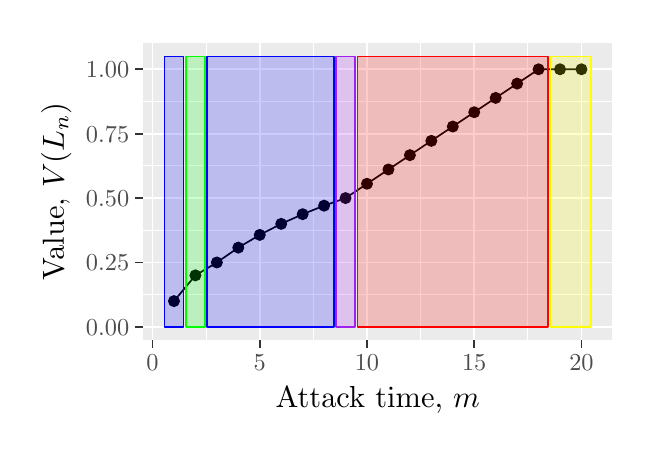
\begin{tikzpicture}[x=1pt,y=1pt]
\definecolor{fillColor}{RGB}{255,255,255}
\path[use as bounding box,fill=fillColor,fill opacity=0.00] (0,0) rectangle (216.81,144.54);
\begin{scope}
\path[clip] (  0.00,  0.00) rectangle (216.81,144.54);
\definecolor{drawColor}{RGB}{255,255,255}
\definecolor{fillColor}{RGB}{255,255,255}

\path[draw=drawColor,line width= 0.6pt,line join=round,line cap=round,fill=fillColor] (  0.00,  0.00) rectangle (216.81,144.54);
\end{scope}
\begin{scope}
\path[clip] ( 41.67, 31.53) rectangle (211.31,139.04);
\definecolor{fillColor}{gray}{0.92}

\path[fill=fillColor] ( 41.67, 31.53) rectangle (211.31,139.04);
\definecolor{drawColor}{RGB}{255,255,255}

\path[draw=drawColor,line width= 0.3pt,line join=round] ( 41.67, 48.05) --
	(211.31, 48.05);

\path[draw=drawColor,line width= 0.3pt,line join=round] ( 41.67, 71.32) --
	(211.31, 71.32);

\path[draw=drawColor,line width= 0.3pt,line join=round] ( 41.67, 94.59) --
	(211.31, 94.59);

\path[draw=drawColor,line width= 0.3pt,line join=round] ( 41.67,117.86) --
	(211.31,117.86);

\path[draw=drawColor,line width= 0.3pt,line join=round] ( 64.49, 31.53) --
	( 64.49,139.04);

\path[draw=drawColor,line width= 0.3pt,line join=round] (103.24, 31.53) --
	(103.24,139.04);

\path[draw=drawColor,line width= 0.3pt,line join=round] (141.99, 31.53) --
	(141.99,139.04);

\path[draw=drawColor,line width= 0.3pt,line join=round] (180.74, 31.53) --
	(180.74,139.04);

\path[draw=drawColor,line width= 0.6pt,line join=round] ( 41.67, 36.42) --
	(211.31, 36.42);

\path[draw=drawColor,line width= 0.6pt,line join=round] ( 41.67, 59.69) --
	(211.31, 59.69);

\path[draw=drawColor,line width= 0.6pt,line join=round] ( 41.67, 82.96) --
	(211.31, 82.96);

\path[draw=drawColor,line width= 0.6pt,line join=round] ( 41.67,106.23) --
	(211.31,106.23);

\path[draw=drawColor,line width= 0.6pt,line join=round] ( 41.67,129.50) --
	(211.31,129.50);

\path[draw=drawColor,line width= 0.6pt,line join=round] ( 45.11, 31.53) --
	( 45.11,139.04);

\path[draw=drawColor,line width= 0.6pt,line join=round] ( 83.86, 31.53) --
	( 83.86,139.04);

\path[draw=drawColor,line width= 0.6pt,line join=round] (122.61, 31.53) --
	(122.61,139.04);

\path[draw=drawColor,line width= 0.6pt,line join=round] (161.36, 31.53) --
	(161.36,139.04);

\path[draw=drawColor,line width= 0.6pt,line join=round] (200.11, 31.53) --
	(200.11,139.04);
\definecolor{drawColor}{RGB}{0,0,0}
\definecolor{fillColor}{RGB}{0,0,0}

\path[draw=drawColor,line width= 0.4pt,line join=round,line cap=round,fill=fillColor] (192.36,129.50) circle (  1.96);

\path[draw=drawColor,line width= 0.4pt,line join=round,line cap=round,fill=fillColor] (200.11,129.50) circle (  1.96);

\path[draw=drawColor,line width= 0.4pt,line join=round,line cap=round,fill=fillColor] (122.61, 88.13) circle (  1.96);

\path[draw=drawColor,line width= 0.4pt,line join=round,line cap=round,fill=fillColor] (130.36, 93.30) circle (  1.96);

\path[draw=drawColor,line width= 0.4pt,line join=round,line cap=round,fill=fillColor] (138.11, 98.47) circle (  1.96);

\path[draw=drawColor,line width= 0.4pt,line join=round,line cap=round,fill=fillColor] (145.86,103.64) circle (  1.96);

\path[draw=drawColor,line width= 0.4pt,line join=round,line cap=round,fill=fillColor] (153.61,108.81) circle (  1.96);

\path[draw=drawColor,line width= 0.4pt,line join=round,line cap=round,fill=fillColor] (161.36,113.99) circle (  1.96);

\path[draw=drawColor,line width= 0.4pt,line join=round,line cap=round,fill=fillColor] (169.11,119.16) circle (  1.96);

\path[draw=drawColor,line width= 0.4pt,line join=round,line cap=round,fill=fillColor] (176.86,124.33) circle (  1.96);

\path[draw=drawColor,line width= 0.4pt,line join=round,line cap=round,fill=fillColor] (184.61,129.50) circle (  1.96);

\path[draw=drawColor,line width= 0.4pt,line join=round,line cap=round,fill=fillColor] ( 60.61, 55.03) circle (  1.96);

\path[draw=drawColor,line width= 0.4pt,line join=round,line cap=round,fill=fillColor] (114.86, 82.96) circle (  1.96);

\path[draw=drawColor,line width= 0.4pt,line join=round,line cap=round,fill=fillColor] (107.11, 80.22) circle (  1.96);

\path[draw=drawColor,line width= 0.4pt,line join=round,line cap=round,fill=fillColor] ( 68.36, 59.69) circle (  1.96);

\path[draw=drawColor,line width= 0.4pt,line join=round,line cap=round,fill=fillColor] ( 76.11, 65.06) circle (  1.96);

\path[draw=drawColor,line width= 0.4pt,line join=round,line cap=round,fill=fillColor] ( 83.86, 69.66) circle (  1.96);

\path[draw=drawColor,line width= 0.4pt,line join=round,line cap=round,fill=fillColor] ( 91.61, 73.65) circle (  1.96);

\path[draw=drawColor,line width= 0.4pt,line join=round,line cap=round,fill=fillColor] ( 99.36, 77.14) circle (  1.96);

\path[draw=drawColor,line width= 0.4pt,line join=round,line cap=round,fill=fillColor] ( 52.86, 45.73) circle (  1.96);

\path[draw=drawColor,line width= 0.6pt,line join=round] ( 52.86, 45.73) --
	( 60.61, 55.03) --
	( 68.36, 59.69) --
	( 76.11, 65.06) --
	( 83.86, 69.66) --
	( 91.61, 73.65) --
	( 99.36, 77.14) --
	(107.11, 80.22) --
	(114.86, 82.96) --
	(122.61, 88.13) --
	(130.36, 93.30) --
	(138.11, 98.47) --
	(145.86,103.64) --
	(153.61,108.81) --
	(161.36,113.99) --
	(169.11,119.16) --
	(176.86,124.33) --
	(184.61,129.50) --
	(192.36,129.50) --
	(200.11,129.50);
\definecolor{drawColor}{RGB}{255,255,0}
\definecolor{fillColor}{RGB}{255,255,0}

\path[draw=drawColor,line width= 0.6pt,line join=round,fill=fillColor,fill opacity=0.20] (188.87, 36.42) rectangle (203.60,134.15);
\definecolor{drawColor}{RGB}{255,0,0}
\definecolor{fillColor}{RGB}{255,0,0}

\path[draw=drawColor,line width= 0.6pt,line join=round,fill=fillColor,fill opacity=0.20] (119.13, 36.42) rectangle (188.10,134.15);
\definecolor{drawColor}{RGB}{160,32,240}
\definecolor{fillColor}{RGB}{160,32,240}

\path[draw=drawColor,line width= 0.6pt,line join=round,fill=fillColor,fill opacity=0.20] (111.38, 36.42) rectangle (118.35,134.15);
\definecolor{drawColor}{RGB}{0,0,255}
\definecolor{fillColor}{RGB}{0,0,255}

\path[draw=drawColor,line width= 0.6pt,line join=round,fill=fillColor,fill opacity=0.20] ( 64.88, 36.42) rectangle (110.60,134.15);
\definecolor{drawColor}{RGB}{0,255,0}
\definecolor{fillColor}{RGB}{0,255,0}

\path[draw=drawColor,line width= 0.6pt,line join=round,fill=fillColor,fill opacity=0.20] ( 57.13, 36.42) rectangle ( 64.10,134.15);
\definecolor{drawColor}{RGB}{0,0,255}
\definecolor{fillColor}{RGB}{0,0,255}

\path[draw=drawColor,line width= 0.6pt,line join=round,fill=fillColor,fill opacity=0.20] ( 49.38, 36.42) rectangle ( 56.35,134.15);
\end{scope}
\begin{scope}
\path[clip] (  0.00,  0.00) rectangle (216.81,144.54);
\definecolor{drawColor}{gray}{0.30}

\node[text=drawColor,anchor=base east,inner sep=0pt, outer sep=0pt, scale=  0.88] at ( 36.72, 33.39) {0.00};

\node[text=drawColor,anchor=base east,inner sep=0pt, outer sep=0pt, scale=  0.88] at ( 36.72, 56.66) {0.25};

\node[text=drawColor,anchor=base east,inner sep=0pt, outer sep=0pt, scale=  0.88] at ( 36.72, 79.93) {0.50};

\node[text=drawColor,anchor=base east,inner sep=0pt, outer sep=0pt, scale=  0.88] at ( 36.72,103.20) {0.75};

\node[text=drawColor,anchor=base east,inner sep=0pt, outer sep=0pt, scale=  0.88] at ( 36.72,126.47) {1.00};
\end{scope}
\begin{scope}
\path[clip] (  0.00,  0.00) rectangle (216.81,144.54);
\definecolor{drawColor}{gray}{0.20}

\path[draw=drawColor,line width= 0.6pt,line join=round] ( 38.92, 36.42) --
	( 41.67, 36.42);

\path[draw=drawColor,line width= 0.6pt,line join=round] ( 38.92, 59.69) --
	( 41.67, 59.69);

\path[draw=drawColor,line width= 0.6pt,line join=round] ( 38.92, 82.96) --
	( 41.67, 82.96);

\path[draw=drawColor,line width= 0.6pt,line join=round] ( 38.92,106.23) --
	( 41.67,106.23);

\path[draw=drawColor,line width= 0.6pt,line join=round] ( 38.92,129.50) --
	( 41.67,129.50);
\end{scope}
\begin{scope}
\path[clip] (  0.00,  0.00) rectangle (216.81,144.54);
\definecolor{drawColor}{gray}{0.20}

\path[draw=drawColor,line width= 0.6pt,line join=round] ( 45.11, 28.78) --
	( 45.11, 31.53);

\path[draw=drawColor,line width= 0.6pt,line join=round] ( 83.86, 28.78) --
	( 83.86, 31.53);

\path[draw=drawColor,line width= 0.6pt,line join=round] (122.61, 28.78) --
	(122.61, 31.53);

\path[draw=drawColor,line width= 0.6pt,line join=round] (161.36, 28.78) --
	(161.36, 31.53);

\path[draw=drawColor,line width= 0.6pt,line join=round] (200.11, 28.78) --
	(200.11, 31.53);
\end{scope}
\begin{scope}
\path[clip] (  0.00,  0.00) rectangle (216.81,144.54);
\definecolor{drawColor}{gray}{0.30}

\node[text=drawColor,anchor=base,inner sep=0pt, outer sep=0pt, scale=  0.88] at ( 45.11, 20.52) {0};

\node[text=drawColor,anchor=base,inner sep=0pt, outer sep=0pt, scale=  0.88] at ( 83.86, 20.52) {5};

\node[text=drawColor,anchor=base,inner sep=0pt, outer sep=0pt, scale=  0.88] at (122.61, 20.52) {10};

\node[text=drawColor,anchor=base,inner sep=0pt, outer sep=0pt, scale=  0.88] at (161.36, 20.52) {15};

\node[text=drawColor,anchor=base,inner sep=0pt, outer sep=0pt, scale=  0.88] at (200.11, 20.52) {20};
\end{scope}
\begin{scope}
\path[clip] (  0.00,  0.00) rectangle (216.81,144.54);
\definecolor{drawColor}{RGB}{0,0,0}

\node[text=drawColor,anchor=base,inner sep=0pt, outer sep=0pt, scale=  1.10] at (126.49,  7.44) {Attack time, $m$};
\end{scope}
\begin{scope}
\path[clip] (  0.00,  0.00) rectangle (216.81,144.54);
\definecolor{drawColor}{RGB}{0,0,0}

\node[text=drawColor,rotate= 90.00,anchor=base,inner sep=0pt, outer sep=0pt, scale=  1.10] at ( 13.08, 85.29) {Value, $V(L_{n})$};
\end{scope}
\end{tikzpicture}
}
      \caption{Value of the line graph, $L_{10}$}
      \end{figure}
      \end{minipage}


    \end{columns}


\end{frame}

\begin{frame}{Strategies used in the second region}
Focusing in on \textcolor{red}{$n-1 < m \leq 2(n-1)$}. We will look at the strategies used to get the bounds $V \leq \frac{m}{2(n-1)}$ and $V \geq \frac{m}{2(n-1)}$.

\begin{itemize}
\item Patroller Strategy, $\bm{\pi}_{H}$, the embedded random Hamiltonian patrol.
\item Attacker Strategy, $\bm{\phi}_{D}$, the diametric attack.
\end{itemize}

\end{frame}

\begin{frame}{Embedded patrols}
An \textcolor{blue}{embedded random Hamiltonian patrol, $\bm{\pi}_{H}$}, is made by `expanding' the line to be Hamiltonian (meaning every non-end node becomes two nodes).

That is the patroller looks at $C_{2(n-1)}$ instead of $L_{n}$, then we get a bound of $V(C_{2(n-1)})=\frac{m}{2(n-1)}$. Now \textcolor{blue}{the patroller cannot do worse in $L_{n}$ than in $C_{2(n-1)}$}, so a lower bound of $V \geq \frac{m}{2(n-1)} $ is achieved.

\begin{figure}
\begin{center}
\resizebox{\textwidth}{!}{
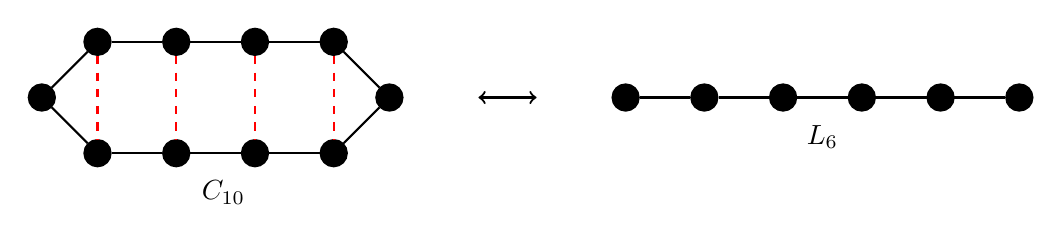
\begin{tikzpicture}[baseline=(current bounding box.north),-,auto,node distance=1cm,
                    thick,main node/.style={circle,draw,fill=black,font=\sffamily\bfseries}]

  \node[main node] (1) {};
  \node[main node] (2) [above right of=1] {};
  \node[main node] (3) [right of=2] {};
  \node[main node] (4) [right of=3] {};
  \node[main node] (5) [right of=4] {};
  \node[main node] (6) [below right of=5] {};
  \node[main node] (7) [below right of=1] {};
  \node[main node] (8) [right of=7] {};
  \node[main node] (9) [right of=8] {};
  \node[main node] (10) [right of=9] {};
  
  \node (P1) [right of=6] {};
  \node (P2) [right of=P1] {};
  
  \node[main node] (a) [right of=P2] {};
  \node[main node] (b) [right of=a] {};
  \node[main node] (c) [right of=b] {};
  \node[main node] (d) [right of=c] {};
  \node[main node] (e) [right of=d] {};
  \node[main node] (f) [right of=e] {};
  
  \draw[<->] (P1) edge (P2);
  

  \path[every node/.style={font=\sffamily}]
    (1) edge  (2)
    edge (7)
    (2) edge (3)
    (3) edge (4)
    (4) edge (5)
    (5) edge (6)
    (6) edge (10)
    (7) edge (8)
    (8) edge (9)
    (9) edge (10)
    (a) edge (b)
    (b) edge (c)
    (c) edge (d)
    (d) edge (e)
    edge (f);
    
     \path[dashed,thick,red,every node/.style={font=\sffamily}]
    (2) edge  (7)
    (3) edge (8)
    (4) edge  (9)
    (5) edge  (10);
    
  
\node [shift={(0.6,-0.5)}] at (8) {$C_{10}$};
\node [shift={(0.5,-0.5)}] at (c) {$L_{6}$};   
\end{tikzpicture}
}
\end{center}
\caption{$C_{10}$ and $L_{6}$ relation by node expanding and simplification.}
\end{figure}
\end{frame}

\begin{frame}{Diametric attack}
Let \textcolor{purple}{$d(i,i')$ be the distance between nodes $i$ and $i'$} with the distance measured by the minimum number of edges.

\begin{definition}[Graph Diameter]
The diameter of a graph $Q$ is defined by $\bar{d}=\max\limits_{i,i' \in N} d(i,i')$ . The node pairs, $(i,i')$, satisfying this are called diametrical.
\end{definition}

A \textcolor{red}{diametric attack, $\bm{\phi}_{D}$} is made by attacking the pair of diametric nodes $1$ and $n$ (the ends), starting with equal probability at every available start time. It is stated to give $V \leq \min\{\frac{1}{2},\frac{m}{2(n-1)}\}= \left\{
\begin{array}{l} 
\frac{1}{2} \text{, if } m<n-1 \\
\frac{m}{2(n-1)} \text{, if } n-1 \leq m \leq 2(n-1),
\end{array}
\right.$ however....
\end{frame}

\section[]{Problem with the diametric strategy}
\hypertarget{Problem with diametric strategy}{}
\begin{frame}{Counter-example for diametric attack}

In the region of $n-1 \leq m \leq 2(n-1)$ the proposed bound is $V \leq \frac{m}{2(n-1)}$. However a simple counter-example shows the bound to be false.
\newline
\newline
\textbf{Counter-example.}
Consider $L_{5}$ with $T=m=5$ , then the patroller only needs to walk between the end nodes to win.
\begin{center}
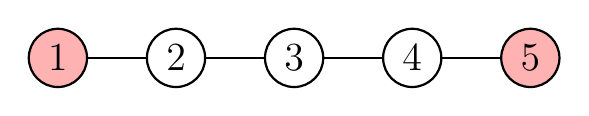
\begin{tikzpicture}[-,auto,node distance=1.5cm,
                    thick,main node/.style={circle,fill=white,draw,font=\sffamily\Large\bfseries}]

  \node[main node,fill=red!30] (1) {$1$};
  \node[main node] (2) [right of=1] {$2$};
  \node[main node] (3) [right of=2]  {$3$};
  \node[main node] (4) [right of=3]  {$4$};
  \node[main node,fill=red!30] (5) [right of=4] {$5$};

  \path[every node/.style={font=\sffamily}]
    (1) edge (2)
    (2) edge (3)
    (3) edge (4)
    (4) edge (5)
    ;
\end{tikzpicture}
\end{center}
The walk $\{ 1,2,3,4,5 \}$ guarantees the capture of all attacks made.

\end{frame}

\begin{frame}{\insertsection}

\textbf{Example.}
Consider $L_{31}$ with $m=45$

\begin{figure}
%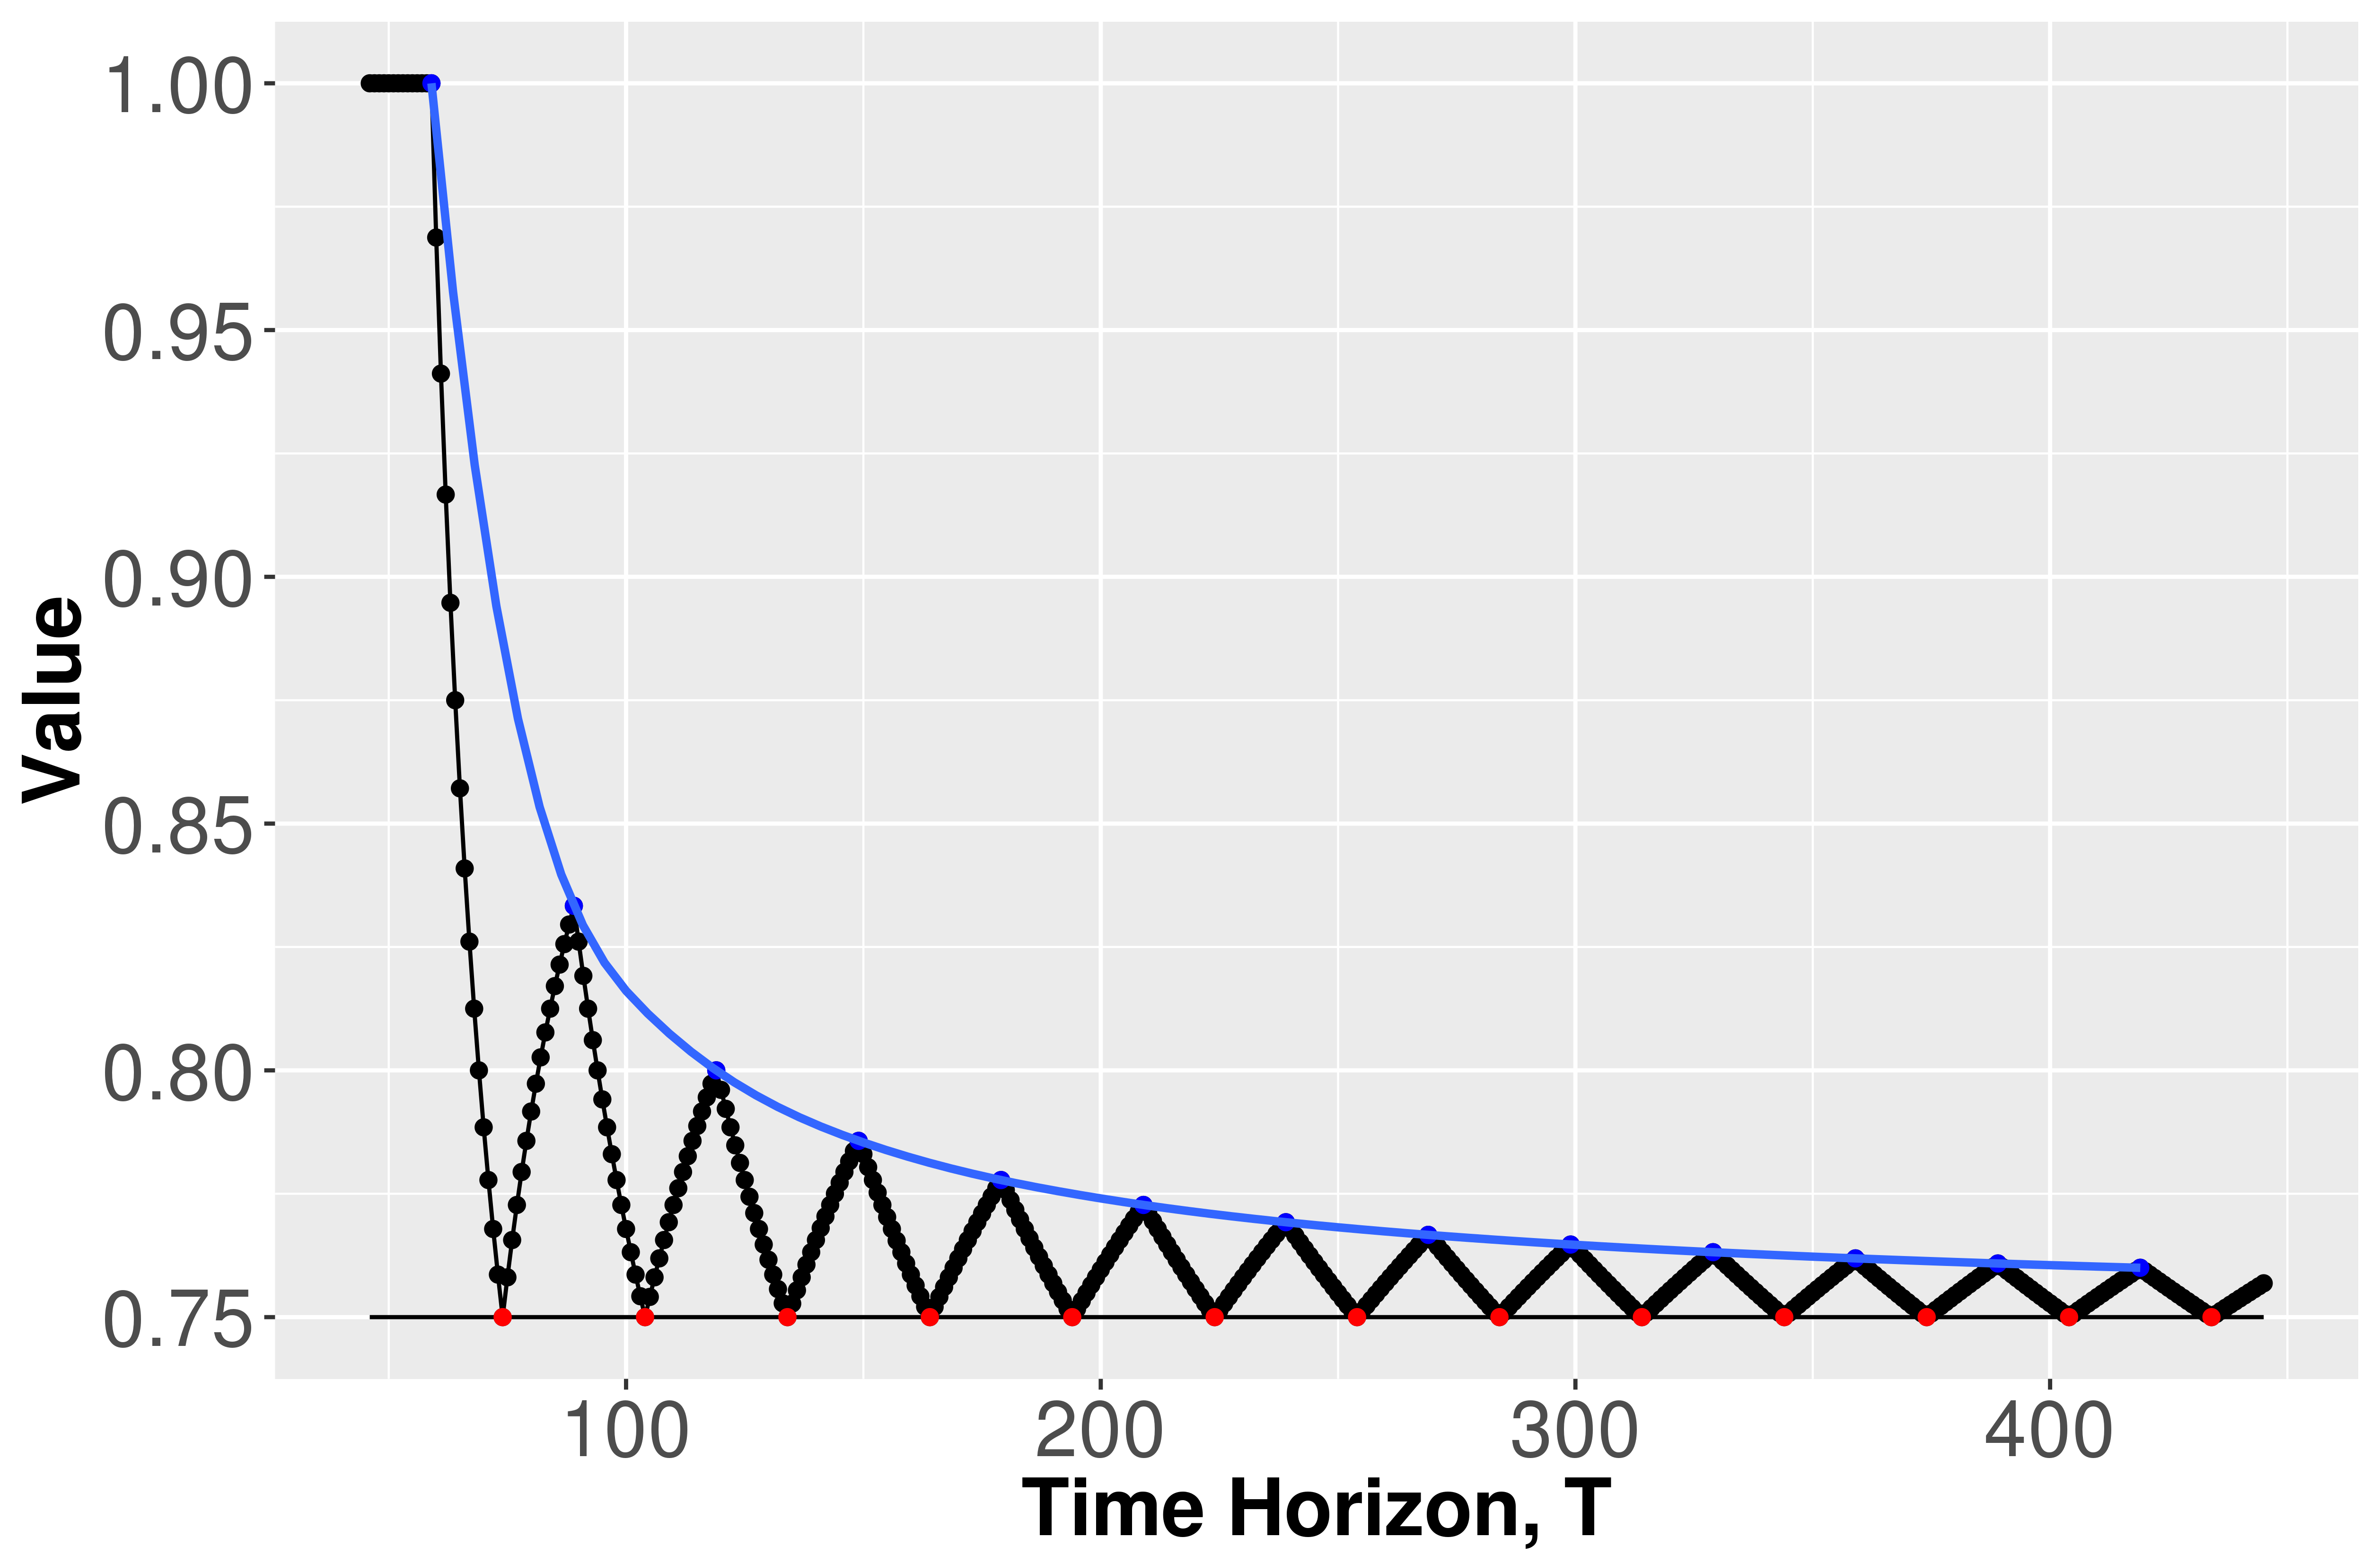
\includegraphics[scale=0.4]{DiametricAttack(m_45,d_30)1.png}
\resizebox{0.95\linewidth}{!}{
% Created by tikzDevice version 0.10.1 on 2017-11-09 12:03:49
% !TEX encoding = UTF-8 Unicode
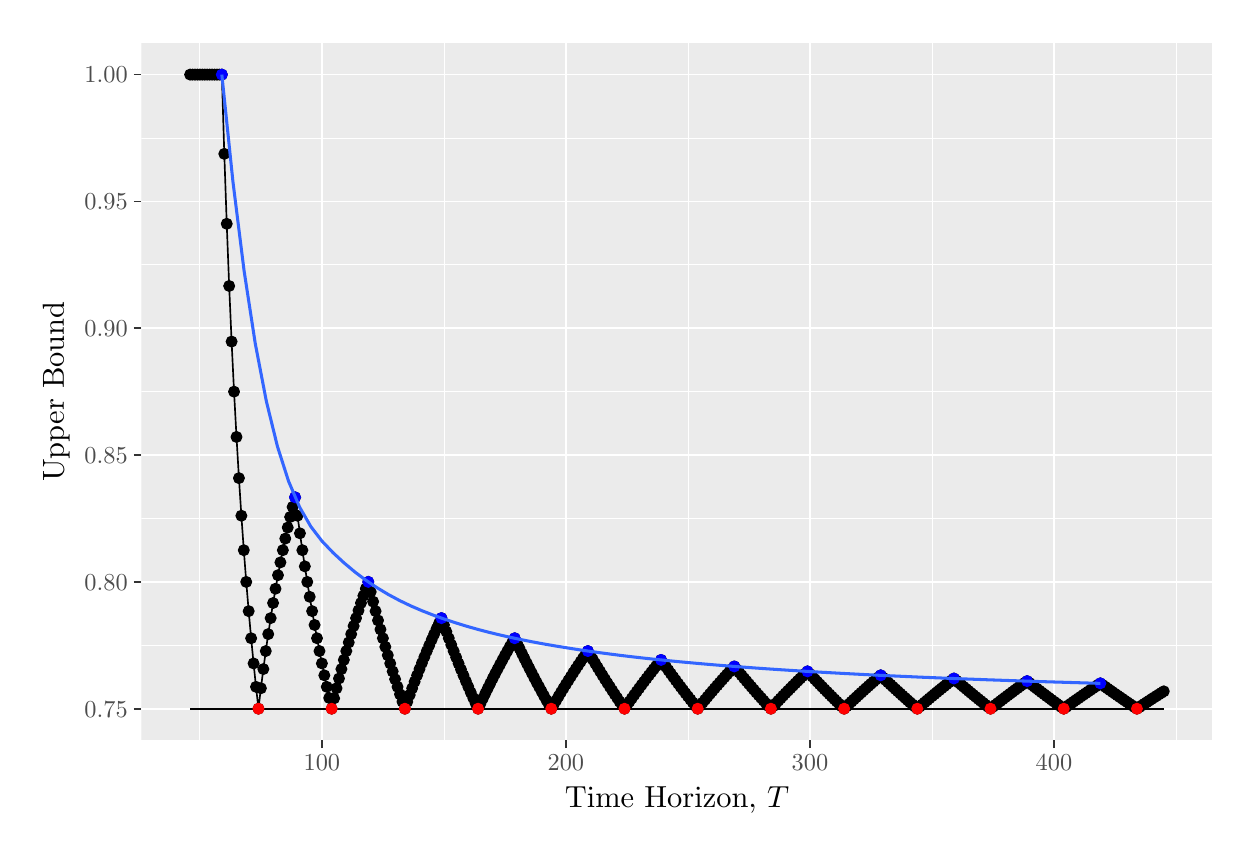
\begin{tikzpicture}[x=1pt,y=1pt]
\definecolor{fillColor}{RGB}{255,255,255}
\path[use as bounding box,fill=fillColor,fill opacity=0.00] (0,0) rectangle (433.62,289.08);
\begin{scope}
\path[clip] (  0.00,  0.00) rectangle (433.62,289.08);
\definecolor{drawColor}{RGB}{255,255,255}
\definecolor{fillColor}{RGB}{255,255,255}

\path[draw=drawColor,line width= 0.6pt,line join=round,line cap=round,fill=fillColor] (  0.00,  0.00) rectangle (433.62,289.08);
\end{scope}
\begin{scope}
\path[clip] ( 41.11, 31.53) rectangle (428.12,283.58);
\definecolor{fillColor}{gray}{0.92}

\path[fill=fillColor] ( 41.11, 31.53) rectangle (428.12,283.58);
\definecolor{drawColor}{RGB}{255,255,255}

\path[draw=drawColor,line width= 0.3pt,line join=round] ( 41.11, 65.90) --
	(428.12, 65.90);

\path[draw=drawColor,line width= 0.3pt,line join=round] ( 41.11,111.73) --
	(428.12,111.73);

\path[draw=drawColor,line width= 0.3pt,line join=round] ( 41.11,157.56) --
	(428.12,157.56);

\path[draw=drawColor,line width= 0.3pt,line join=round] ( 41.11,203.38) --
	(428.12,203.38);

\path[draw=drawColor,line width= 0.3pt,line join=round] ( 41.11,249.21) --
	(428.12,249.21);

\path[draw=drawColor,line width= 0.3pt,line join=round] ( 62.23, 31.53) --
	( 62.23,283.58);

\path[draw=drawColor,line width= 0.3pt,line join=round] (150.41, 31.53) --
	(150.41,283.58);

\path[draw=drawColor,line width= 0.3pt,line join=round] (238.58, 31.53) --
	(238.58,283.58);

\path[draw=drawColor,line width= 0.3pt,line join=round] (326.76, 31.53) --
	(326.76,283.58);

\path[draw=drawColor,line width= 0.3pt,line join=round] (414.94, 31.53) --
	(414.94,283.58);

\path[draw=drawColor,line width= 0.6pt,line join=round] ( 41.11, 42.99) --
	(428.12, 42.99);

\path[draw=drawColor,line width= 0.6pt,line join=round] ( 41.11, 88.81) --
	(428.12, 88.81);

\path[draw=drawColor,line width= 0.6pt,line join=round] ( 41.11,134.64) --
	(428.12,134.64);

\path[draw=drawColor,line width= 0.6pt,line join=round] ( 41.11,180.47) --
	(428.12,180.47);

\path[draw=drawColor,line width= 0.6pt,line join=round] ( 41.11,226.30) --
	(428.12,226.30);

\path[draw=drawColor,line width= 0.6pt,line join=round] ( 41.11,272.12) --
	(428.12,272.12);

\path[draw=drawColor,line width= 0.6pt,line join=round] (106.32, 31.53) --
	(106.32,283.58);

\path[draw=drawColor,line width= 0.6pt,line join=round] (194.49, 31.53) --
	(194.49,283.58);

\path[draw=drawColor,line width= 0.6pt,line join=round] (282.67, 31.53) --
	(282.67,283.58);

\path[draw=drawColor,line width= 0.6pt,line join=round] (370.85, 31.53) --
	(370.85,283.58);
\definecolor{drawColor}{RGB}{0,0,0}
\definecolor{fillColor}{RGB}{0,0,0}

\path[draw=drawColor,line width= 0.4pt,line join=round,line cap=round,fill=fillColor] ( 58.70,272.12) circle (  1.96);

\path[draw=drawColor,line width= 0.4pt,line join=round,line cap=round,fill=fillColor] ( 59.58,272.12) circle (  1.96);

\path[draw=drawColor,line width= 0.4pt,line join=round,line cap=round,fill=fillColor] ( 60.47,272.12) circle (  1.96);

\path[draw=drawColor,line width= 0.4pt,line join=round,line cap=round,fill=fillColor] ( 61.35,272.12) circle (  1.96);

\path[draw=drawColor,line width= 0.4pt,line join=round,line cap=round,fill=fillColor] ( 62.23,272.12) circle (  1.96);

\path[draw=drawColor,line width= 0.4pt,line join=round,line cap=round,fill=fillColor] ( 63.11,272.12) circle (  1.96);

\path[draw=drawColor,line width= 0.4pt,line join=round,line cap=round,fill=fillColor] ( 63.99,272.12) circle (  1.96);

\path[draw=drawColor,line width= 0.4pt,line join=round,line cap=round,fill=fillColor] ( 64.87,272.12) circle (  1.96);

\path[draw=drawColor,line width= 0.4pt,line join=round,line cap=round,fill=fillColor] ( 65.76,272.12) circle (  1.96);

\path[draw=drawColor,line width= 0.4pt,line join=round,line cap=round,fill=fillColor] ( 66.64,272.12) circle (  1.96);

\path[draw=drawColor,line width= 0.4pt,line join=round,line cap=round,fill=fillColor] ( 67.52,272.12) circle (  1.96);

\path[draw=drawColor,line width= 0.4pt,line join=round,line cap=round,fill=fillColor] ( 68.40,272.12) circle (  1.96);

\path[draw=drawColor,line width= 0.4pt,line join=round,line cap=round,fill=fillColor] ( 69.28,272.12) circle (  1.96);

\path[draw=drawColor,line width= 0.4pt,line join=round,line cap=round,fill=fillColor] ( 70.16,272.12) circle (  1.96);

\path[draw=drawColor,line width= 0.4pt,line join=round,line cap=round,fill=fillColor] ( 71.05,243.48) circle (  1.96);

\path[draw=drawColor,line width= 0.4pt,line join=round,line cap=round,fill=fillColor] ( 71.93,218.21) circle (  1.96);

\path[draw=drawColor,line width= 0.4pt,line join=round,line cap=round,fill=fillColor] ( 72.81,195.74) circle (  1.96);

\path[draw=drawColor,line width= 0.4pt,line join=round,line cap=round,fill=fillColor] ( 73.69,175.65) circle (  1.96);

\path[draw=drawColor,line width= 0.4pt,line join=round,line cap=round,fill=fillColor] ( 74.57,157.56) circle (  1.96);

\path[draw=drawColor,line width= 0.4pt,line join=round,line cap=round,fill=fillColor] ( 75.46,141.19) circle (  1.96);

\path[draw=drawColor,line width= 0.4pt,line join=round,line cap=round,fill=fillColor] ( 76.34,126.31) circle (  1.96);

\path[draw=drawColor,line width= 0.4pt,line join=round,line cap=round,fill=fillColor] ( 77.22,112.72) circle (  1.96);

\path[draw=drawColor,line width= 0.4pt,line join=round,line cap=round,fill=fillColor] ( 78.10,100.27) circle (  1.96);

\path[draw=drawColor,line width= 0.4pt,line join=round,line cap=round,fill=fillColor] ( 78.98, 88.81) circle (  1.96);

\path[draw=drawColor,line width= 0.4pt,line join=round,line cap=round,fill=fillColor] ( 79.86, 78.24) circle (  1.96);

\path[draw=drawColor,line width= 0.4pt,line join=round,line cap=round,fill=fillColor] ( 80.75, 68.45) circle (  1.96);

\path[draw=drawColor,line width= 0.4pt,line join=round,line cap=round,fill=fillColor] ( 81.63, 59.35) circle (  1.96);

\path[draw=drawColor,line width= 0.4pt,line join=round,line cap=round,fill=fillColor] ( 82.51, 50.89) circle (  1.96);

\path[draw=drawColor,line width= 0.4pt,line join=round,line cap=round,fill=fillColor] ( 83.39, 42.99) circle (  1.96);

\path[draw=drawColor,line width= 0.4pt,line join=round,line cap=round,fill=fillColor] ( 84.27, 50.38) circle (  1.96);

\path[draw=drawColor,line width= 0.4pt,line join=round,line cap=round,fill=fillColor] ( 85.16, 57.31) circle (  1.96);

\path[draw=drawColor,line width= 0.4pt,line join=round,line cap=round,fill=fillColor] ( 86.04, 63.82) circle (  1.96);

\path[draw=drawColor,line width= 0.4pt,line join=round,line cap=round,fill=fillColor] ( 86.92, 69.94) circle (  1.96);

\path[draw=drawColor,line width= 0.4pt,line join=round,line cap=round,fill=fillColor] ( 87.80, 75.72) circle (  1.96);

\path[draw=drawColor,line width= 0.4pt,line join=round,line cap=round,fill=fillColor] ( 88.68, 81.18) circle (  1.96);

\path[draw=drawColor,line width= 0.4pt,line join=round,line cap=round,fill=fillColor] ( 89.56, 86.34) circle (  1.96);

\path[draw=drawColor,line width= 0.4pt,line join=round,line cap=round,fill=fillColor] ( 90.45, 91.23) circle (  1.96);

\path[draw=drawColor,line width= 0.4pt,line join=round,line cap=round,fill=fillColor] ( 91.33, 95.86) circle (  1.96);

\path[draw=drawColor,line width= 0.4pt,line join=round,line cap=round,fill=fillColor] ( 92.21,100.27) circle (  1.96);

\path[draw=drawColor,line width= 0.4pt,line join=round,line cap=round,fill=fillColor] ( 93.09,104.46) circle (  1.96);

\path[draw=drawColor,line width= 0.4pt,line join=round,line cap=round,fill=fillColor] ( 93.97,108.45) circle (  1.96);

\path[draw=drawColor,line width= 0.4pt,line join=round,line cap=round,fill=fillColor] ( 94.85,112.26) circle (  1.96);

\path[draw=drawColor,line width= 0.4pt,line join=round,line cap=round,fill=fillColor] ( 95.74,115.89) circle (  1.96);

\path[draw=drawColor,line width= 0.4pt,line join=round,line cap=round,fill=fillColor] ( 96.62,119.37) circle (  1.96);

\path[draw=drawColor,line width= 0.4pt,line join=round,line cap=round,fill=fillColor] ( 97.50,112.72) circle (  1.96);

\path[draw=drawColor,line width= 0.4pt,line join=round,line cap=round,fill=fillColor] ( 98.38,106.37) circle (  1.96);

\path[draw=drawColor,line width= 0.4pt,line join=round,line cap=round,fill=fillColor] ( 99.26,100.27) circle (  1.96);

\path[draw=drawColor,line width= 0.4pt,line join=round,line cap=round,fill=fillColor] (100.15, 94.43) circle (  1.96);

\path[draw=drawColor,line width= 0.4pt,line join=round,line cap=round,fill=fillColor] (101.03, 88.81) circle (  1.96);

\path[draw=drawColor,line width= 0.4pt,line join=round,line cap=round,fill=fillColor] (101.91, 83.42) circle (  1.96);

\path[draw=drawColor,line width= 0.4pt,line join=round,line cap=round,fill=fillColor] (102.79, 78.24) circle (  1.96);

\path[draw=drawColor,line width= 0.4pt,line join=round,line cap=round,fill=fillColor] (103.67, 73.25) circle (  1.96);

\path[draw=drawColor,line width= 0.4pt,line join=round,line cap=round,fill=fillColor] (104.55, 68.45) circle (  1.96);

\path[draw=drawColor,line width= 0.4pt,line join=round,line cap=round,fill=fillColor] (105.44, 63.82) circle (  1.96);

\path[draw=drawColor,line width= 0.4pt,line join=round,line cap=round,fill=fillColor] (106.32, 59.35) circle (  1.96);

\path[draw=drawColor,line width= 0.4pt,line join=round,line cap=round,fill=fillColor] (107.20, 55.05) circle (  1.96);

\path[draw=drawColor,line width= 0.4pt,line join=round,line cap=round,fill=fillColor] (108.08, 50.89) circle (  1.96);

\path[draw=drawColor,line width= 0.4pt,line join=round,line cap=round,fill=fillColor] (108.96, 46.87) circle (  1.96);

\path[draw=drawColor,line width= 0.4pt,line join=round,line cap=round,fill=fillColor] (109.84, 42.99) circle (  1.96);

\path[draw=drawColor,line width= 0.4pt,line join=round,line cap=round,fill=fillColor] (110.73, 46.74) circle (  1.96);

\path[draw=drawColor,line width= 0.4pt,line join=round,line cap=round,fill=fillColor] (111.61, 50.38) circle (  1.96);

\path[draw=drawColor,line width= 0.4pt,line join=round,line cap=round,fill=fillColor] (112.49, 53.90) circle (  1.96);

\path[draw=drawColor,line width= 0.4pt,line join=round,line cap=round,fill=fillColor] (113.37, 57.31) circle (  1.96);

\path[draw=drawColor,line width= 0.4pt,line join=round,line cap=round,fill=fillColor] (114.25, 60.61) circle (  1.96);

\path[draw=drawColor,line width= 0.4pt,line join=round,line cap=round,fill=fillColor] (115.14, 63.82) circle (  1.96);

\path[draw=drawColor,line width= 0.4pt,line join=round,line cap=round,fill=fillColor] (116.02, 66.93) circle (  1.96);

\path[draw=drawColor,line width= 0.4pt,line join=round,line cap=round,fill=fillColor] (116.90, 69.94) circle (  1.96);

\path[draw=drawColor,line width= 0.4pt,line join=round,line cap=round,fill=fillColor] (117.78, 72.87) circle (  1.96);

\path[draw=drawColor,line width= 0.4pt,line join=round,line cap=round,fill=fillColor] (118.66, 75.72) circle (  1.96);

\path[draw=drawColor,line width= 0.4pt,line join=round,line cap=round,fill=fillColor] (119.54, 78.49) circle (  1.96);

\path[draw=drawColor,line width= 0.4pt,line join=round,line cap=round,fill=fillColor] (120.43, 81.18) circle (  1.96);

\path[draw=drawColor,line width= 0.4pt,line join=round,line cap=round,fill=fillColor] (121.31, 83.79) circle (  1.96);

\path[draw=drawColor,line width= 0.4pt,line join=round,line cap=round,fill=fillColor] (122.19, 86.34) circle (  1.96);

\path[draw=drawColor,line width= 0.4pt,line join=round,line cap=round,fill=fillColor] (123.07, 88.81) circle (  1.96);

\path[draw=drawColor,line width= 0.4pt,line join=round,line cap=round,fill=fillColor] (123.95, 85.20) circle (  1.96);

\path[draw=drawColor,line width= 0.4pt,line join=round,line cap=round,fill=fillColor] (124.83, 81.67) circle (  1.96);

\path[draw=drawColor,line width= 0.4pt,line join=round,line cap=round,fill=fillColor] (125.72, 78.24) circle (  1.96);

\path[draw=drawColor,line width= 0.4pt,line join=round,line cap=round,fill=fillColor] (126.60, 74.89) circle (  1.96);

\path[draw=drawColor,line width= 0.4pt,line join=round,line cap=round,fill=fillColor] (127.48, 71.63) circle (  1.96);

\path[draw=drawColor,line width= 0.4pt,line join=round,line cap=round,fill=fillColor] (128.36, 68.45) circle (  1.96);

\path[draw=drawColor,line width= 0.4pt,line join=round,line cap=round,fill=fillColor] (129.24, 65.34) circle (  1.96);

\path[draw=drawColor,line width= 0.4pt,line join=round,line cap=round,fill=fillColor] (130.13, 62.31) circle (  1.96);

\path[draw=drawColor,line width= 0.4pt,line join=round,line cap=round,fill=fillColor] (131.01, 59.35) circle (  1.96);

\path[draw=drawColor,line width= 0.4pt,line join=round,line cap=round,fill=fillColor] (131.89, 56.47) circle (  1.96);

\path[draw=drawColor,line width= 0.4pt,line join=round,line cap=round,fill=fillColor] (132.77, 53.64) circle (  1.96);

\path[draw=drawColor,line width= 0.4pt,line join=round,line cap=round,fill=fillColor] (133.65, 50.89) circle (  1.96);

\path[draw=drawColor,line width= 0.4pt,line join=round,line cap=round,fill=fillColor] (134.53, 48.20) circle (  1.96);

\path[draw=drawColor,line width= 0.4pt,line join=round,line cap=round,fill=fillColor] (135.42, 45.56) circle (  1.96);

\path[draw=drawColor,line width= 0.4pt,line join=round,line cap=round,fill=fillColor] (136.30, 42.99) circle (  1.96);

\path[draw=drawColor,line width= 0.4pt,line join=round,line cap=round,fill=fillColor] (137.18, 45.51) circle (  1.96);

\path[draw=drawColor,line width= 0.4pt,line join=round,line cap=round,fill=fillColor] (138.06, 47.97) circle (  1.96);

\path[draw=drawColor,line width= 0.4pt,line join=round,line cap=round,fill=fillColor] (138.94, 50.38) circle (  1.96);

\path[draw=drawColor,line width= 0.4pt,line join=round,line cap=round,fill=fillColor] (139.82, 52.74) circle (  1.96);

\path[draw=drawColor,line width= 0.4pt,line join=round,line cap=round,fill=fillColor] (140.71, 55.05) circle (  1.96);

\path[draw=drawColor,line width= 0.4pt,line join=round,line cap=round,fill=fillColor] (141.59, 57.31) circle (  1.96);

\path[draw=drawColor,line width= 0.4pt,line join=round,line cap=round,fill=fillColor] (142.47, 59.52) circle (  1.96);

\path[draw=drawColor,line width= 0.4pt,line join=round,line cap=round,fill=fillColor] (143.35, 61.69) circle (  1.96);

\path[draw=drawColor,line width= 0.4pt,line join=round,line cap=round,fill=fillColor] (144.23, 63.82) circle (  1.96);

\path[draw=drawColor,line width= 0.4pt,line join=round,line cap=round,fill=fillColor] (145.12, 65.90) circle (  1.96);

\path[draw=drawColor,line width= 0.4pt,line join=round,line cap=round,fill=fillColor] (146.00, 67.94) circle (  1.96);

\path[draw=drawColor,line width= 0.4pt,line join=round,line cap=round,fill=fillColor] (146.88, 69.94) circle (  1.96);

\path[draw=drawColor,line width= 0.4pt,line join=round,line cap=round,fill=fillColor] (147.76, 71.91) circle (  1.96);

\path[draw=drawColor,line width= 0.4pt,line join=round,line cap=round,fill=fillColor] (148.64, 73.83) circle (  1.96);

\path[draw=drawColor,line width= 0.4pt,line join=round,line cap=round,fill=fillColor] (149.52, 75.72) circle (  1.96);

\path[draw=drawColor,line width= 0.4pt,line join=round,line cap=round,fill=fillColor] (150.41, 73.25) circle (  1.96);

\path[draw=drawColor,line width= 0.4pt,line join=round,line cap=round,fill=fillColor] (151.29, 70.83) circle (  1.96);

\path[draw=drawColor,line width= 0.4pt,line join=round,line cap=round,fill=fillColor] (152.17, 68.45) circle (  1.96);

\path[draw=drawColor,line width= 0.4pt,line join=round,line cap=round,fill=fillColor] (153.05, 66.11) circle (  1.96);

\path[draw=drawColor,line width= 0.4pt,line join=round,line cap=round,fill=fillColor] (153.93, 63.82) circle (  1.96);

\path[draw=drawColor,line width= 0.4pt,line join=round,line cap=round,fill=fillColor] (154.82, 61.57) circle (  1.96);

\path[draw=drawColor,line width= 0.4pt,line join=round,line cap=round,fill=fillColor] (155.70, 59.35) circle (  1.96);

\path[draw=drawColor,line width= 0.4pt,line join=round,line cap=round,fill=fillColor] (156.58, 57.18) circle (  1.96);

\path[draw=drawColor,line width= 0.4pt,line join=round,line cap=round,fill=fillColor] (157.46, 55.05) circle (  1.96);

\path[draw=drawColor,line width= 0.4pt,line join=round,line cap=round,fill=fillColor] (158.34, 52.95) circle (  1.96);

\path[draw=drawColor,line width= 0.4pt,line join=round,line cap=round,fill=fillColor] (159.22, 50.89) circle (  1.96);

\path[draw=drawColor,line width= 0.4pt,line join=round,line cap=round,fill=fillColor] (160.11, 48.86) circle (  1.96);

\path[draw=drawColor,line width= 0.4pt,line join=round,line cap=round,fill=fillColor] (160.99, 46.87) circle (  1.96);

\path[draw=drawColor,line width= 0.4pt,line join=round,line cap=round,fill=fillColor] (161.87, 44.91) circle (  1.96);

\path[draw=drawColor,line width= 0.4pt,line join=round,line cap=round,fill=fillColor] (162.75, 42.99) circle (  1.96);

\path[draw=drawColor,line width= 0.4pt,line join=round,line cap=round,fill=fillColor] (163.63, 44.88) circle (  1.96);

\path[draw=drawColor,line width= 0.4pt,line join=round,line cap=round,fill=fillColor] (164.51, 46.74) circle (  1.96);

\path[draw=drawColor,line width= 0.4pt,line join=round,line cap=round,fill=fillColor] (165.40, 48.58) circle (  1.96);

\path[draw=drawColor,line width= 0.4pt,line join=round,line cap=round,fill=fillColor] (166.28, 50.38) circle (  1.96);

\path[draw=drawColor,line width= 0.4pt,line join=round,line cap=round,fill=fillColor] (167.16, 52.15) circle (  1.96);

\path[draw=drawColor,line width= 0.4pt,line join=round,line cap=round,fill=fillColor] (168.04, 53.90) circle (  1.96);

\path[draw=drawColor,line width= 0.4pt,line join=round,line cap=round,fill=fillColor] (168.92, 55.62) circle (  1.96);

\path[draw=drawColor,line width= 0.4pt,line join=round,line cap=round,fill=fillColor] (169.81, 57.31) circle (  1.96);

\path[draw=drawColor,line width= 0.4pt,line join=round,line cap=round,fill=fillColor] (170.69, 58.97) circle (  1.96);

\path[draw=drawColor,line width= 0.4pt,line join=round,line cap=round,fill=fillColor] (171.57, 60.61) circle (  1.96);

\path[draw=drawColor,line width= 0.4pt,line join=round,line cap=round,fill=fillColor] (172.45, 62.23) circle (  1.96);

\path[draw=drawColor,line width= 0.4pt,line join=round,line cap=round,fill=fillColor] (173.33, 63.82) circle (  1.96);

\path[draw=drawColor,line width= 0.4pt,line join=round,line cap=round,fill=fillColor] (174.21, 65.38) circle (  1.96);

\path[draw=drawColor,line width= 0.4pt,line join=round,line cap=round,fill=fillColor] (175.10, 66.93) circle (  1.96);

\path[draw=drawColor,line width= 0.4pt,line join=round,line cap=round,fill=fillColor] (175.98, 68.45) circle (  1.96);

\path[draw=drawColor,line width= 0.4pt,line join=round,line cap=round,fill=fillColor] (176.86, 66.57) circle (  1.96);

\path[draw=drawColor,line width= 0.4pt,line join=round,line cap=round,fill=fillColor] (177.74, 64.73) circle (  1.96);

\path[draw=drawColor,line width= 0.4pt,line join=round,line cap=round,fill=fillColor] (178.62, 62.91) circle (  1.96);

\path[draw=drawColor,line width= 0.4pt,line join=round,line cap=round,fill=fillColor] (179.50, 61.12) circle (  1.96);

\path[draw=drawColor,line width= 0.4pt,line join=round,line cap=round,fill=fillColor] (180.39, 59.35) circle (  1.96);

\path[draw=drawColor,line width= 0.4pt,line join=round,line cap=round,fill=fillColor] (181.27, 57.61) circle (  1.96);

\path[draw=drawColor,line width= 0.4pt,line join=round,line cap=round,fill=fillColor] (182.15, 55.90) circle (  1.96);

\path[draw=drawColor,line width= 0.4pt,line join=round,line cap=round,fill=fillColor] (183.03, 54.20) circle (  1.96);

\path[draw=drawColor,line width= 0.4pt,line join=round,line cap=round,fill=fillColor] (183.91, 52.53) circle (  1.96);

\path[draw=drawColor,line width= 0.4pt,line join=round,line cap=round,fill=fillColor] (184.80, 50.89) circle (  1.96);

\path[draw=drawColor,line width= 0.4pt,line join=round,line cap=round,fill=fillColor] (185.68, 49.27) circle (  1.96);

\path[draw=drawColor,line width= 0.4pt,line join=round,line cap=round,fill=fillColor] (186.56, 47.66) circle (  1.96);

\path[draw=drawColor,line width= 0.4pt,line join=round,line cap=round,fill=fillColor] (187.44, 46.08) circle (  1.96);

\path[draw=drawColor,line width= 0.4pt,line join=round,line cap=round,fill=fillColor] (188.32, 44.53) circle (  1.96);

\path[draw=drawColor,line width= 0.4pt,line join=round,line cap=round,fill=fillColor] (189.20, 42.99) circle (  1.96);

\path[draw=drawColor,line width= 0.4pt,line join=round,line cap=round,fill=fillColor] (190.09, 44.50) circle (  1.96);

\path[draw=drawColor,line width= 0.4pt,line join=round,line cap=round,fill=fillColor] (190.97, 46.00) circle (  1.96);

\path[draw=drawColor,line width= 0.4pt,line join=round,line cap=round,fill=fillColor] (191.85, 47.48) circle (  1.96);

\path[draw=drawColor,line width= 0.4pt,line join=round,line cap=round,fill=fillColor] (192.73, 48.94) circle (  1.96);

\path[draw=drawColor,line width= 0.4pt,line join=round,line cap=round,fill=fillColor] (193.61, 50.38) circle (  1.96);

\path[draw=drawColor,line width= 0.4pt,line join=round,line cap=round,fill=fillColor] (194.49, 51.80) circle (  1.96);

\path[draw=drawColor,line width= 0.4pt,line join=round,line cap=round,fill=fillColor] (195.38, 53.20) circle (  1.96);

\path[draw=drawColor,line width= 0.4pt,line join=round,line cap=round,fill=fillColor] (196.26, 54.59) circle (  1.96);

\path[draw=drawColor,line width= 0.4pt,line join=round,line cap=round,fill=fillColor] (197.14, 55.96) circle (  1.96);

\path[draw=drawColor,line width= 0.4pt,line join=round,line cap=round,fill=fillColor] (198.02, 57.31) circle (  1.96);

\path[draw=drawColor,line width= 0.4pt,line join=round,line cap=round,fill=fillColor] (198.90, 58.64) circle (  1.96);

\path[draw=drawColor,line width= 0.4pt,line join=round,line cap=round,fill=fillColor] (199.79, 59.96) circle (  1.96);

\path[draw=drawColor,line width= 0.4pt,line join=round,line cap=round,fill=fillColor] (200.67, 61.26) circle (  1.96);

\path[draw=drawColor,line width= 0.4pt,line join=round,line cap=round,fill=fillColor] (201.55, 62.55) circle (  1.96);

\path[draw=drawColor,line width= 0.4pt,line join=round,line cap=round,fill=fillColor] (202.43, 63.82) circle (  1.96);

\path[draw=drawColor,line width= 0.4pt,line join=round,line cap=round,fill=fillColor] (203.31, 62.31) circle (  1.96);

\path[draw=drawColor,line width= 0.4pt,line join=round,line cap=round,fill=fillColor] (204.19, 60.82) circle (  1.96);

\path[draw=drawColor,line width= 0.4pt,line join=round,line cap=round,fill=fillColor] (205.08, 59.35) circle (  1.96);

\path[draw=drawColor,line width= 0.4pt,line join=round,line cap=round,fill=fillColor] (205.96, 57.90) circle (  1.96);

\path[draw=drawColor,line width= 0.4pt,line join=round,line cap=round,fill=fillColor] (206.84, 56.47) circle (  1.96);

\path[draw=drawColor,line width= 0.4pt,line join=round,line cap=round,fill=fillColor] (207.72, 55.05) circle (  1.96);

\path[draw=drawColor,line width= 0.4pt,line join=round,line cap=round,fill=fillColor] (208.60, 53.64) circle (  1.96);

\path[draw=drawColor,line width= 0.4pt,line join=round,line cap=round,fill=fillColor] (209.48, 52.26) circle (  1.96);

\path[draw=drawColor,line width= 0.4pt,line join=round,line cap=round,fill=fillColor] (210.37, 50.89) circle (  1.96);

\path[draw=drawColor,line width= 0.4pt,line join=round,line cap=round,fill=fillColor] (211.25, 49.53) circle (  1.96);

\path[draw=drawColor,line width= 0.4pt,line join=round,line cap=round,fill=fillColor] (212.13, 48.20) circle (  1.96);

\path[draw=drawColor,line width= 0.4pt,line join=round,line cap=round,fill=fillColor] (213.01, 46.87) circle (  1.96);

\path[draw=drawColor,line width= 0.4pt,line join=round,line cap=round,fill=fillColor] (213.89, 45.56) circle (  1.96);

\path[draw=drawColor,line width= 0.4pt,line join=round,line cap=round,fill=fillColor] (214.78, 44.27) circle (  1.96);

\path[draw=drawColor,line width= 0.4pt,line join=round,line cap=round,fill=fillColor] (215.66, 42.99) circle (  1.96);

\path[draw=drawColor,line width= 0.4pt,line join=round,line cap=round,fill=fillColor] (216.54, 44.25) circle (  1.96);

\path[draw=drawColor,line width= 0.4pt,line join=round,line cap=round,fill=fillColor] (217.42, 45.51) circle (  1.96);

\path[draw=drawColor,line width= 0.4pt,line join=round,line cap=round,fill=fillColor] (218.30, 46.74) circle (  1.96);

\path[draw=drawColor,line width= 0.4pt,line join=round,line cap=round,fill=fillColor] (219.18, 47.97) circle (  1.96);

\path[draw=drawColor,line width= 0.4pt,line join=round,line cap=round,fill=fillColor] (220.07, 49.18) circle (  1.96);

\path[draw=drawColor,line width= 0.4pt,line join=round,line cap=round,fill=fillColor] (220.95, 50.38) circle (  1.96);

\path[draw=drawColor,line width= 0.4pt,line join=round,line cap=round,fill=fillColor] (221.83, 51.56) circle (  1.96);

\path[draw=drawColor,line width= 0.4pt,line join=round,line cap=round,fill=fillColor] (222.71, 52.74) circle (  1.96);

\path[draw=drawColor,line width= 0.4pt,line join=round,line cap=round,fill=fillColor] (223.59, 53.90) circle (  1.96);

\path[draw=drawColor,line width= 0.4pt,line join=round,line cap=round,fill=fillColor] (224.47, 55.05) circle (  1.96);

\path[draw=drawColor,line width= 0.4pt,line join=round,line cap=round,fill=fillColor] (225.36, 56.18) circle (  1.96);

\path[draw=drawColor,line width= 0.4pt,line join=round,line cap=round,fill=fillColor] (226.24, 57.31) circle (  1.96);

\path[draw=drawColor,line width= 0.4pt,line join=round,line cap=round,fill=fillColor] (227.12, 58.42) circle (  1.96);

\path[draw=drawColor,line width= 0.4pt,line join=round,line cap=round,fill=fillColor] (228.00, 59.52) circle (  1.96);

\path[draw=drawColor,line width= 0.4pt,line join=round,line cap=round,fill=fillColor] (228.88, 60.61) circle (  1.96);

\path[draw=drawColor,line width= 0.4pt,line join=round,line cap=round,fill=fillColor] (229.77, 59.35) circle (  1.96);

\path[draw=drawColor,line width= 0.4pt,line join=round,line cap=round,fill=fillColor] (230.65, 58.11) circle (  1.96);

\path[draw=drawColor,line width= 0.4pt,line join=round,line cap=round,fill=fillColor] (231.53, 56.87) circle (  1.96);

\path[draw=drawColor,line width= 0.4pt,line join=round,line cap=round,fill=fillColor] (232.41, 55.65) circle (  1.96);

\path[draw=drawColor,line width= 0.4pt,line join=round,line cap=round,fill=fillColor] (233.29, 54.44) circle (  1.96);

\path[draw=drawColor,line width= 0.4pt,line join=round,line cap=round,fill=fillColor] (234.17, 53.25) circle (  1.96);

\path[draw=drawColor,line width= 0.4pt,line join=round,line cap=round,fill=fillColor] (235.06, 52.06) circle (  1.96);

\path[draw=drawColor,line width= 0.4pt,line join=round,line cap=round,fill=fillColor] (235.94, 50.89) circle (  1.96);

\path[draw=drawColor,line width= 0.4pt,line join=round,line cap=round,fill=fillColor] (236.82, 49.73) circle (  1.96);

\path[draw=drawColor,line width= 0.4pt,line join=round,line cap=round,fill=fillColor] (237.70, 48.58) circle (  1.96);

\path[draw=drawColor,line width= 0.4pt,line join=round,line cap=round,fill=fillColor] (238.58, 47.44) circle (  1.96);

\path[draw=drawColor,line width= 0.4pt,line join=round,line cap=round,fill=fillColor] (239.47, 46.31) circle (  1.96);

\path[draw=drawColor,line width= 0.4pt,line join=round,line cap=round,fill=fillColor] (240.35, 45.19) circle (  1.96);

\path[draw=drawColor,line width= 0.4pt,line join=round,line cap=round,fill=fillColor] (241.23, 44.08) circle (  1.96);

\path[draw=drawColor,line width= 0.4pt,line join=round,line cap=round,fill=fillColor] (242.11, 42.99) circle (  1.96);

\path[draw=drawColor,line width= 0.4pt,line join=round,line cap=round,fill=fillColor] (242.99, 44.07) circle (  1.96);

\path[draw=drawColor,line width= 0.4pt,line join=round,line cap=round,fill=fillColor] (243.87, 45.15) circle (  1.96);

\path[draw=drawColor,line width= 0.4pt,line join=round,line cap=round,fill=fillColor] (244.76, 46.21) circle (  1.96);

\path[draw=drawColor,line width= 0.4pt,line join=round,line cap=round,fill=fillColor] (245.64, 47.27) circle (  1.96);

\path[draw=drawColor,line width= 0.4pt,line join=round,line cap=round,fill=fillColor] (246.52, 48.32) circle (  1.96);

\path[draw=drawColor,line width= 0.4pt,line join=round,line cap=round,fill=fillColor] (247.40, 49.35) circle (  1.96);

\path[draw=drawColor,line width= 0.4pt,line join=round,line cap=round,fill=fillColor] (248.28, 50.38) circle (  1.96);

\path[draw=drawColor,line width= 0.4pt,line join=round,line cap=round,fill=fillColor] (249.16, 51.40) circle (  1.96);

\path[draw=drawColor,line width= 0.4pt,line join=round,line cap=round,fill=fillColor] (250.05, 52.40) circle (  1.96);

\path[draw=drawColor,line width= 0.4pt,line join=round,line cap=round,fill=fillColor] (250.93, 53.40) circle (  1.96);

\path[draw=drawColor,line width= 0.4pt,line join=round,line cap=round,fill=fillColor] (251.81, 54.39) circle (  1.96);

\path[draw=drawColor,line width= 0.4pt,line join=round,line cap=round,fill=fillColor] (252.69, 55.37) circle (  1.96);

\path[draw=drawColor,line width= 0.4pt,line join=round,line cap=round,fill=fillColor] (253.57, 56.35) circle (  1.96);

\path[draw=drawColor,line width= 0.4pt,line join=round,line cap=round,fill=fillColor] (254.46, 57.31) circle (  1.96);

\path[draw=drawColor,line width= 0.4pt,line join=round,line cap=round,fill=fillColor] (255.34, 58.26) circle (  1.96);

\path[draw=drawColor,line width= 0.4pt,line join=round,line cap=round,fill=fillColor] (256.22, 57.18) circle (  1.96);

\path[draw=drawColor,line width= 0.4pt,line join=round,line cap=round,fill=fillColor] (257.10, 56.11) circle (  1.96);

\path[draw=drawColor,line width= 0.4pt,line join=round,line cap=round,fill=fillColor] (257.98, 55.05) circle (  1.96);

\path[draw=drawColor,line width= 0.4pt,line join=round,line cap=round,fill=fillColor] (258.86, 53.99) circle (  1.96);

\path[draw=drawColor,line width= 0.4pt,line join=round,line cap=round,fill=fillColor] (259.75, 52.95) circle (  1.96);

\path[draw=drawColor,line width= 0.4pt,line join=round,line cap=round,fill=fillColor] (260.63, 51.91) circle (  1.96);

\path[draw=drawColor,line width= 0.4pt,line join=round,line cap=round,fill=fillColor] (261.51, 50.89) circle (  1.96);

\path[draw=drawColor,line width= 0.4pt,line join=round,line cap=round,fill=fillColor] (262.39, 49.87) circle (  1.96);

\path[draw=drawColor,line width= 0.4pt,line join=round,line cap=round,fill=fillColor] (263.27, 48.86) circle (  1.96);

\path[draw=drawColor,line width= 0.4pt,line join=round,line cap=round,fill=fillColor] (264.15, 47.86) circle (  1.96);

\path[draw=drawColor,line width= 0.4pt,line join=round,line cap=round,fill=fillColor] (265.04, 46.87) circle (  1.96);

\path[draw=drawColor,line width= 0.4pt,line join=round,line cap=round,fill=fillColor] (265.92, 45.89) circle (  1.96);

\path[draw=drawColor,line width= 0.4pt,line join=round,line cap=round,fill=fillColor] (266.80, 44.91) circle (  1.96);

\path[draw=drawColor,line width= 0.4pt,line join=round,line cap=round,fill=fillColor] (267.68, 43.95) circle (  1.96);

\path[draw=drawColor,line width= 0.4pt,line join=round,line cap=round,fill=fillColor] (268.56, 42.99) circle (  1.96);

\path[draw=drawColor,line width= 0.4pt,line join=round,line cap=round,fill=fillColor] (269.45, 43.94) circle (  1.96);

\path[draw=drawColor,line width= 0.4pt,line join=round,line cap=round,fill=fillColor] (270.33, 44.88) circle (  1.96);

\path[draw=drawColor,line width= 0.4pt,line join=round,line cap=round,fill=fillColor] (271.21, 45.82) circle (  1.96);

\path[draw=drawColor,line width= 0.4pt,line join=round,line cap=round,fill=fillColor] (272.09, 46.74) circle (  1.96);

\path[draw=drawColor,line width= 0.4pt,line join=round,line cap=round,fill=fillColor] (272.97, 47.66) circle (  1.96);

\path[draw=drawColor,line width= 0.4pt,line join=round,line cap=round,fill=fillColor] (273.85, 48.58) circle (  1.96);

\path[draw=drawColor,line width= 0.4pt,line join=round,line cap=round,fill=fillColor] (274.74, 49.48) circle (  1.96);

\path[draw=drawColor,line width= 0.4pt,line join=round,line cap=round,fill=fillColor] (275.62, 50.38) circle (  1.96);

\path[draw=drawColor,line width= 0.4pt,line join=round,line cap=round,fill=fillColor] (276.50, 51.27) circle (  1.96);

\path[draw=drawColor,line width= 0.4pt,line join=round,line cap=round,fill=fillColor] (277.38, 52.15) circle (  1.96);

\path[draw=drawColor,line width= 0.4pt,line join=round,line cap=round,fill=fillColor] (278.26, 53.03) circle (  1.96);

\path[draw=drawColor,line width= 0.4pt,line join=round,line cap=round,fill=fillColor] (279.14, 53.90) circle (  1.96);

\path[draw=drawColor,line width= 0.4pt,line join=round,line cap=round,fill=fillColor] (280.03, 54.76) circle (  1.96);

\path[draw=drawColor,line width= 0.4pt,line join=round,line cap=round,fill=fillColor] (280.91, 55.62) circle (  1.96);

\path[draw=drawColor,line width= 0.4pt,line join=round,line cap=round,fill=fillColor] (281.79, 56.47) circle (  1.96);

\path[draw=drawColor,line width= 0.4pt,line join=round,line cap=round,fill=fillColor] (282.67, 55.52) circle (  1.96);

\path[draw=drawColor,line width= 0.4pt,line join=round,line cap=round,fill=fillColor] (283.55, 54.58) circle (  1.96);

\path[draw=drawColor,line width= 0.4pt,line join=round,line cap=round,fill=fillColor] (284.44, 53.64) circle (  1.96);

\path[draw=drawColor,line width= 0.4pt,line join=round,line cap=round,fill=fillColor] (285.32, 52.72) circle (  1.96);

\path[draw=drawColor,line width= 0.4pt,line join=round,line cap=round,fill=fillColor] (286.20, 51.80) circle (  1.96);

\path[draw=drawColor,line width= 0.4pt,line join=round,line cap=round,fill=fillColor] (287.08, 50.89) circle (  1.96);

\path[draw=drawColor,line width= 0.4pt,line join=round,line cap=round,fill=fillColor] (287.96, 49.98) circle (  1.96);

\path[draw=drawColor,line width= 0.4pt,line join=round,line cap=round,fill=fillColor] (288.84, 49.09) circle (  1.96);

\path[draw=drawColor,line width= 0.4pt,line join=round,line cap=round,fill=fillColor] (289.73, 48.20) circle (  1.96);

\path[draw=drawColor,line width= 0.4pt,line join=round,line cap=round,fill=fillColor] (290.61, 47.31) circle (  1.96);

\path[draw=drawColor,line width= 0.4pt,line join=round,line cap=round,fill=fillColor] (291.49, 46.43) circle (  1.96);

\path[draw=drawColor,line width= 0.4pt,line join=round,line cap=round,fill=fillColor] (292.37, 45.56) circle (  1.96);

\path[draw=drawColor,line width= 0.4pt,line join=round,line cap=round,fill=fillColor] (293.25, 44.70) circle (  1.96);

\path[draw=drawColor,line width= 0.4pt,line join=round,line cap=round,fill=fillColor] (294.13, 43.84) circle (  1.96);

\path[draw=drawColor,line width= 0.4pt,line join=round,line cap=round,fill=fillColor] (295.02, 42.99) circle (  1.96);

\path[draw=drawColor,line width= 0.4pt,line join=round,line cap=round,fill=fillColor] (295.90, 43.83) circle (  1.96);

\path[draw=drawColor,line width= 0.4pt,line join=round,line cap=round,fill=fillColor] (296.78, 44.67) circle (  1.96);

\path[draw=drawColor,line width= 0.4pt,line join=round,line cap=round,fill=fillColor] (297.66, 45.51) circle (  1.96);

\path[draw=drawColor,line width= 0.4pt,line join=round,line cap=round,fill=fillColor] (298.54, 46.33) circle (  1.96);

\path[draw=drawColor,line width= 0.4pt,line join=round,line cap=round,fill=fillColor] (299.43, 47.15) circle (  1.96);

\path[draw=drawColor,line width= 0.4pt,line join=round,line cap=round,fill=fillColor] (300.31, 47.97) circle (  1.96);

\path[draw=drawColor,line width= 0.4pt,line join=round,line cap=round,fill=fillColor] (301.19, 48.78) circle (  1.96);

\path[draw=drawColor,line width= 0.4pt,line join=round,line cap=round,fill=fillColor] (302.07, 49.58) circle (  1.96);

\path[draw=drawColor,line width= 0.4pt,line join=round,line cap=round,fill=fillColor] (302.95, 50.38) circle (  1.96);

\path[draw=drawColor,line width= 0.4pt,line join=round,line cap=round,fill=fillColor] (303.83, 51.17) circle (  1.96);

\path[draw=drawColor,line width= 0.4pt,line join=round,line cap=round,fill=fillColor] (304.72, 51.96) circle (  1.96);

\path[draw=drawColor,line width= 0.4pt,line join=round,line cap=round,fill=fillColor] (305.60, 52.74) circle (  1.96);

\path[draw=drawColor,line width= 0.4pt,line join=round,line cap=round,fill=fillColor] (306.48, 53.51) circle (  1.96);

\path[draw=drawColor,line width= 0.4pt,line join=round,line cap=round,fill=fillColor] (307.36, 54.28) circle (  1.96);

\path[draw=drawColor,line width= 0.4pt,line join=round,line cap=round,fill=fillColor] (308.24, 55.05) circle (  1.96);

\path[draw=drawColor,line width= 0.4pt,line join=round,line cap=round,fill=fillColor] (309.12, 54.20) circle (  1.96);

\path[draw=drawColor,line width= 0.4pt,line join=round,line cap=round,fill=fillColor] (310.01, 53.37) circle (  1.96);

\path[draw=drawColor,line width= 0.4pt,line join=round,line cap=round,fill=fillColor] (310.89, 52.53) circle (  1.96);

\path[draw=drawColor,line width= 0.4pt,line join=round,line cap=round,fill=fillColor] (311.77, 51.71) circle (  1.96);

\path[draw=drawColor,line width= 0.4pt,line join=round,line cap=round,fill=fillColor] (312.65, 50.89) circle (  1.96);

\path[draw=drawColor,line width= 0.4pt,line join=round,line cap=round,fill=fillColor] (313.53, 50.07) circle (  1.96);

\path[draw=drawColor,line width= 0.4pt,line join=round,line cap=round,fill=fillColor] (314.42, 49.27) circle (  1.96);

\path[draw=drawColor,line width= 0.4pt,line join=round,line cap=round,fill=fillColor] (315.30, 48.46) circle (  1.96);

\path[draw=drawColor,line width= 0.4pt,line join=round,line cap=round,fill=fillColor] (316.18, 47.66) circle (  1.96);

\path[draw=drawColor,line width= 0.4pt,line join=round,line cap=round,fill=fillColor] (317.06, 46.87) circle (  1.96);

\path[draw=drawColor,line width= 0.4pt,line join=round,line cap=round,fill=fillColor] (317.94, 46.08) circle (  1.96);

\path[draw=drawColor,line width= 0.4pt,line join=round,line cap=round,fill=fillColor] (318.82, 45.30) circle (  1.96);

\path[draw=drawColor,line width= 0.4pt,line join=round,line cap=round,fill=fillColor] (319.71, 44.53) circle (  1.96);

\path[draw=drawColor,line width= 0.4pt,line join=round,line cap=round,fill=fillColor] (320.59, 43.75) circle (  1.96);

\path[draw=drawColor,line width= 0.4pt,line join=round,line cap=round,fill=fillColor] (321.47, 42.99) circle (  1.96);

\path[draw=drawColor,line width= 0.4pt,line join=round,line cap=round,fill=fillColor] (322.35, 43.75) circle (  1.96);

\path[draw=drawColor,line width= 0.4pt,line join=round,line cap=round,fill=fillColor] (323.23, 44.50) circle (  1.96);

\path[draw=drawColor,line width= 0.4pt,line join=round,line cap=round,fill=fillColor] (324.12, 45.26) circle (  1.96);

\path[draw=drawColor,line width= 0.4pt,line join=round,line cap=round,fill=fillColor] (325.00, 46.00) circle (  1.96);

\path[draw=drawColor,line width= 0.4pt,line join=round,line cap=round,fill=fillColor] (325.88, 46.74) circle (  1.96);

\path[draw=drawColor,line width= 0.4pt,line join=round,line cap=round,fill=fillColor] (326.76, 47.48) circle (  1.96);

\path[draw=drawColor,line width= 0.4pt,line join=round,line cap=round,fill=fillColor] (327.64, 48.21) circle (  1.96);

\path[draw=drawColor,line width= 0.4pt,line join=round,line cap=round,fill=fillColor] (328.52, 48.94) circle (  1.96);

\path[draw=drawColor,line width= 0.4pt,line join=round,line cap=round,fill=fillColor] (329.41, 49.66) circle (  1.96);

\path[draw=drawColor,line width= 0.4pt,line join=round,line cap=round,fill=fillColor] (330.29, 50.38) circle (  1.96);

\path[draw=drawColor,line width= 0.4pt,line join=round,line cap=round,fill=fillColor] (331.17, 51.09) circle (  1.96);

\path[draw=drawColor,line width= 0.4pt,line join=round,line cap=round,fill=fillColor] (332.05, 51.80) circle (  1.96);

\path[draw=drawColor,line width= 0.4pt,line join=round,line cap=round,fill=fillColor] (332.93, 52.50) circle (  1.96);

\path[draw=drawColor,line width= 0.4pt,line join=round,line cap=round,fill=fillColor] (333.81, 53.20) circle (  1.96);

\path[draw=drawColor,line width= 0.4pt,line join=round,line cap=round,fill=fillColor] (334.70, 53.90) circle (  1.96);

\path[draw=drawColor,line width= 0.4pt,line join=round,line cap=round,fill=fillColor] (335.58, 53.14) circle (  1.96);

\path[draw=drawColor,line width= 0.4pt,line join=round,line cap=round,fill=fillColor] (336.46, 52.38) circle (  1.96);

\path[draw=drawColor,line width= 0.4pt,line join=round,line cap=round,fill=fillColor] (337.34, 51.63) circle (  1.96);

\path[draw=drawColor,line width= 0.4pt,line join=round,line cap=round,fill=fillColor] (338.22, 50.89) circle (  1.96);

\path[draw=drawColor,line width= 0.4pt,line join=round,line cap=round,fill=fillColor] (339.11, 50.15) circle (  1.96);

\path[draw=drawColor,line width= 0.4pt,line join=round,line cap=round,fill=fillColor] (339.99, 49.41) circle (  1.96);

\path[draw=drawColor,line width= 0.4pt,line join=round,line cap=round,fill=fillColor] (340.87, 48.68) circle (  1.96);

\path[draw=drawColor,line width= 0.4pt,line join=round,line cap=round,fill=fillColor] (341.75, 47.95) circle (  1.96);

\path[draw=drawColor,line width= 0.4pt,line join=round,line cap=round,fill=fillColor] (342.63, 47.23) circle (  1.96);

\path[draw=drawColor,line width= 0.4pt,line join=round,line cap=round,fill=fillColor] (343.51, 46.51) circle (  1.96);

\path[draw=drawColor,line width= 0.4pt,line join=round,line cap=round,fill=fillColor] (344.40, 45.80) circle (  1.96);

\path[draw=drawColor,line width= 0.4pt,line join=round,line cap=round,fill=fillColor] (345.28, 45.09) circle (  1.96);

\path[draw=drawColor,line width= 0.4pt,line join=round,line cap=round,fill=fillColor] (346.16, 44.38) circle (  1.96);

\path[draw=drawColor,line width= 0.4pt,line join=round,line cap=round,fill=fillColor] (347.04, 43.68) circle (  1.96);

\path[draw=drawColor,line width= 0.4pt,line join=round,line cap=round,fill=fillColor] (347.92, 42.99) circle (  1.96);

\path[draw=drawColor,line width= 0.4pt,line join=round,line cap=round,fill=fillColor] (348.80, 43.68) circle (  1.96);

\path[draw=drawColor,line width= 0.4pt,line join=round,line cap=round,fill=fillColor] (349.69, 44.37) circle (  1.96);

\path[draw=drawColor,line width= 0.4pt,line join=round,line cap=round,fill=fillColor] (350.57, 45.05) circle (  1.96);

\path[draw=drawColor,line width= 0.4pt,line join=round,line cap=round,fill=fillColor] (351.45, 45.73) circle (  1.96);

\path[draw=drawColor,line width= 0.4pt,line join=round,line cap=round,fill=fillColor] (352.33, 46.41) circle (  1.96);

\path[draw=drawColor,line width= 0.4pt,line join=round,line cap=round,fill=fillColor] (353.21, 47.08) circle (  1.96);

\path[draw=drawColor,line width= 0.4pt,line join=round,line cap=round,fill=fillColor] (354.10, 47.75) circle (  1.96);

\path[draw=drawColor,line width= 0.4pt,line join=round,line cap=round,fill=fillColor] (354.98, 48.41) circle (  1.96);

\path[draw=drawColor,line width= 0.4pt,line join=round,line cap=round,fill=fillColor] (355.86, 49.07) circle (  1.96);

\path[draw=drawColor,line width= 0.4pt,line join=round,line cap=round,fill=fillColor] (356.74, 49.73) circle (  1.96);

\path[draw=drawColor,line width= 0.4pt,line join=round,line cap=round,fill=fillColor] (357.62, 50.38) circle (  1.96);

\path[draw=drawColor,line width= 0.4pt,line join=round,line cap=round,fill=fillColor] (358.50, 51.03) circle (  1.96);

\path[draw=drawColor,line width= 0.4pt,line join=round,line cap=round,fill=fillColor] (359.39, 51.67) circle (  1.96);

\path[draw=drawColor,line width= 0.4pt,line join=round,line cap=round,fill=fillColor] (360.27, 52.31) circle (  1.96);

\path[draw=drawColor,line width= 0.4pt,line join=round,line cap=round,fill=fillColor] (361.15, 52.95) circle (  1.96);

\path[draw=drawColor,line width= 0.4pt,line join=round,line cap=round,fill=fillColor] (362.03, 52.26) circle (  1.96);

\path[draw=drawColor,line width= 0.4pt,line join=round,line cap=round,fill=fillColor] (362.91, 51.57) circle (  1.96);

\path[draw=drawColor,line width= 0.4pt,line join=round,line cap=round,fill=fillColor] (363.79, 50.89) circle (  1.96);

\path[draw=drawColor,line width= 0.4pt,line join=round,line cap=round,fill=fillColor] (364.68, 50.21) circle (  1.96);

\path[draw=drawColor,line width= 0.4pt,line join=round,line cap=round,fill=fillColor] (365.56, 49.53) circle (  1.96);

\path[draw=drawColor,line width= 0.4pt,line join=round,line cap=round,fill=fillColor] (366.44, 48.86) circle (  1.96);

\path[draw=drawColor,line width= 0.4pt,line join=round,line cap=round,fill=fillColor] (367.32, 48.20) circle (  1.96);

\path[draw=drawColor,line width= 0.4pt,line join=round,line cap=round,fill=fillColor] (368.20, 47.53) circle (  1.96);

\path[draw=drawColor,line width= 0.4pt,line join=round,line cap=round,fill=fillColor] (369.09, 46.87) circle (  1.96);

\path[draw=drawColor,line width= 0.4pt,line join=round,line cap=round,fill=fillColor] (369.97, 46.21) circle (  1.96);

\path[draw=drawColor,line width= 0.4pt,line join=round,line cap=round,fill=fillColor] (370.85, 45.56) circle (  1.96);

\path[draw=drawColor,line width= 0.4pt,line join=round,line cap=round,fill=fillColor] (371.73, 44.91) circle (  1.96);

\path[draw=drawColor,line width= 0.4pt,line join=round,line cap=round,fill=fillColor] (372.61, 44.27) circle (  1.96);

\path[draw=drawColor,line width= 0.4pt,line join=round,line cap=round,fill=fillColor] (373.49, 43.63) circle (  1.96);

\path[draw=drawColor,line width= 0.4pt,line join=round,line cap=round,fill=fillColor] (374.38, 42.99) circle (  1.96);

\path[draw=drawColor,line width= 0.4pt,line join=round,line cap=round,fill=fillColor] (375.26, 43.62) circle (  1.96);

\path[draw=drawColor,line width= 0.4pt,line join=round,line cap=round,fill=fillColor] (376.14, 44.25) circle (  1.96);

\path[draw=drawColor,line width= 0.4pt,line join=round,line cap=round,fill=fillColor] (377.02, 44.88) circle (  1.96);

\path[draw=drawColor,line width= 0.4pt,line join=round,line cap=round,fill=fillColor] (377.90, 45.51) circle (  1.96);

\path[draw=drawColor,line width= 0.4pt,line join=round,line cap=round,fill=fillColor] (378.78, 46.13) circle (  1.96);

\path[draw=drawColor,line width= 0.4pt,line join=round,line cap=round,fill=fillColor] (379.67, 46.74) circle (  1.96);

\path[draw=drawColor,line width= 0.4pt,line join=round,line cap=round,fill=fillColor] (380.55, 47.36) circle (  1.96);

\path[draw=drawColor,line width= 0.4pt,line join=round,line cap=round,fill=fillColor] (381.43, 47.97) circle (  1.96);

\path[draw=drawColor,line width= 0.4pt,line join=round,line cap=round,fill=fillColor] (382.31, 48.58) circle (  1.96);

\path[draw=drawColor,line width= 0.4pt,line join=round,line cap=round,fill=fillColor] (383.19, 49.18) circle (  1.96);

\path[draw=drawColor,line width= 0.4pt,line join=round,line cap=round,fill=fillColor] (384.08, 49.78) circle (  1.96);

\path[draw=drawColor,line width= 0.4pt,line join=round,line cap=round,fill=fillColor] (384.96, 50.38) circle (  1.96);

\path[draw=drawColor,line width= 0.4pt,line join=round,line cap=round,fill=fillColor] (385.84, 50.97) circle (  1.96);

\path[draw=drawColor,line width= 0.4pt,line join=round,line cap=round,fill=fillColor] (386.72, 51.56) circle (  1.96);

\path[draw=drawColor,line width= 0.4pt,line join=round,line cap=round,fill=fillColor] (387.60, 52.15) circle (  1.96);

\path[draw=drawColor,line width= 0.4pt,line join=round,line cap=round,fill=fillColor] (388.48, 51.52) circle (  1.96);

\path[draw=drawColor,line width= 0.4pt,line join=round,line cap=round,fill=fillColor] (389.37, 50.89) circle (  1.96);

\path[draw=drawColor,line width= 0.4pt,line join=round,line cap=round,fill=fillColor] (390.25, 50.26) circle (  1.96);

\path[draw=drawColor,line width= 0.4pt,line join=round,line cap=round,fill=fillColor] (391.13, 49.64) circle (  1.96);

\path[draw=drawColor,line width= 0.4pt,line join=round,line cap=round,fill=fillColor] (392.01, 49.02) circle (  1.96);

\path[draw=drawColor,line width= 0.4pt,line join=round,line cap=round,fill=fillColor] (392.89, 48.40) circle (  1.96);

\path[draw=drawColor,line width= 0.4pt,line join=round,line cap=round,fill=fillColor] (393.78, 47.79) circle (  1.96);

\path[draw=drawColor,line width= 0.4pt,line join=round,line cap=round,fill=fillColor] (394.66, 47.18) circle (  1.96);

\path[draw=drawColor,line width= 0.4pt,line join=round,line cap=round,fill=fillColor] (395.54, 46.57) circle (  1.96);

\path[draw=drawColor,line width= 0.4pt,line join=round,line cap=round,fill=fillColor] (396.42, 45.96) circle (  1.96);

\path[draw=drawColor,line width= 0.4pt,line join=round,line cap=round,fill=fillColor] (397.30, 45.36) circle (  1.96);

\path[draw=drawColor,line width= 0.4pt,line join=round,line cap=round,fill=fillColor] (398.18, 44.76) circle (  1.96);

\path[draw=drawColor,line width= 0.4pt,line join=round,line cap=round,fill=fillColor] (399.07, 44.17) circle (  1.96);

\path[draw=drawColor,line width= 0.4pt,line join=round,line cap=round,fill=fillColor] (399.95, 43.58) circle (  1.96);

\path[draw=drawColor,line width= 0.4pt,line join=round,line cap=round,fill=fillColor] (400.83, 42.99) circle (  1.96);

\path[draw=drawColor,line width= 0.4pt,line join=round,line cap=round,fill=fillColor] (401.71, 43.57) circle (  1.96);

\path[draw=drawColor,line width= 0.4pt,line join=round,line cap=round,fill=fillColor] (402.59, 44.16) circle (  1.96);

\path[draw=drawColor,line width= 0.4pt,line join=round,line cap=round,fill=fillColor] (403.47, 44.74) circle (  1.96);

\path[draw=drawColor,line width= 0.4pt,line join=round,line cap=round,fill=fillColor] (404.36, 45.31) circle (  1.96);

\path[draw=drawColor,line width= 0.4pt,line join=round,line cap=round,fill=fillColor] (405.24, 45.89) circle (  1.96);

\path[draw=drawColor,line width= 0.4pt,line join=round,line cap=round,fill=fillColor] (406.12, 46.46) circle (  1.96);

\path[draw=drawColor,line width= 0.4pt,line join=round,line cap=round,fill=fillColor] (407.00, 47.03) circle (  1.96);

\path[draw=drawColor,line width= 0.4pt,line join=round,line cap=round,fill=fillColor] (407.88, 47.59) circle (  1.96);

\path[draw=drawColor,line width= 0.4pt,line join=round,line cap=round,fill=fillColor] (408.77, 48.16) circle (  1.96);

\path[draw=drawColor,line width= 0.4pt,line join=round,line cap=round,fill=fillColor] (409.65, 48.72) circle (  1.96);

\path[draw=drawColor,line width= 0.4pt,line join=round,line cap=round,fill=fillColor] (410.53, 49.27) circle (  1.96);

\path[draw=drawColor,line width= 0.6pt,line join=round] ( 58.70,272.12) --
	( 59.58,272.12) --
	( 60.47,272.12) --
	( 61.35,272.12) --
	( 62.23,272.12) --
	( 63.11,272.12) --
	( 63.99,272.12) --
	( 64.87,272.12) --
	( 65.76,272.12) --
	( 66.64,272.12) --
	( 67.52,272.12) --
	( 68.40,272.12) --
	( 69.28,272.12) --
	( 70.16,272.12) --
	( 71.05,243.48) --
	( 71.93,218.21) --
	( 72.81,195.74) --
	( 73.69,175.65) --
	( 74.57,157.56) --
	( 75.46,141.19) --
	( 76.34,126.31) --
	( 77.22,112.72) --
	( 78.10,100.27) --
	( 78.98, 88.81) --
	( 79.86, 78.24) --
	( 80.75, 68.45) --
	( 81.63, 59.35) --
	( 82.51, 50.89) --
	( 83.39, 42.99) --
	( 84.27, 50.38) --
	( 85.16, 57.31) --
	( 86.04, 63.82) --
	( 86.92, 69.94) --
	( 87.80, 75.72) --
	( 88.68, 81.18) --
	( 89.56, 86.34) --
	( 90.45, 91.23) --
	( 91.33, 95.86) --
	( 92.21,100.27) --
	( 93.09,104.46) --
	( 93.97,108.45) --
	( 94.85,112.26) --
	( 95.74,115.89) --
	( 96.62,119.37) --
	( 97.50,112.72) --
	( 98.38,106.37) --
	( 99.26,100.27) --
	(100.15, 94.43) --
	(101.03, 88.81) --
	(101.91, 83.42) --
	(102.79, 78.24) --
	(103.67, 73.25) --
	(104.55, 68.45) --
	(105.44, 63.82) --
	(106.32, 59.35) --
	(107.20, 55.05) --
	(108.08, 50.89) --
	(108.96, 46.87) --
	(109.84, 42.99) --
	(110.73, 46.74) --
	(111.61, 50.38) --
	(112.49, 53.90) --
	(113.37, 57.31) --
	(114.25, 60.61) --
	(115.14, 63.82) --
	(116.02, 66.93) --
	(116.90, 69.94) --
	(117.78, 72.87) --
	(118.66, 75.72) --
	(119.54, 78.49) --
	(120.43, 81.18) --
	(121.31, 83.79) --
	(122.19, 86.34) --
	(123.07, 88.81) --
	(123.95, 85.20) --
	(124.83, 81.67) --
	(125.72, 78.24) --
	(126.60, 74.89) --
	(127.48, 71.63) --
	(128.36, 68.45) --
	(129.24, 65.34) --
	(130.13, 62.31) --
	(131.01, 59.35) --
	(131.89, 56.47) --
	(132.77, 53.64) --
	(133.65, 50.89) --
	(134.53, 48.20) --
	(135.42, 45.56) --
	(136.30, 42.99) --
	(137.18, 45.51) --
	(138.06, 47.97) --
	(138.94, 50.38) --
	(139.82, 52.74) --
	(140.71, 55.05) --
	(141.59, 57.31) --
	(142.47, 59.52) --
	(143.35, 61.69) --
	(144.23, 63.82) --
	(145.12, 65.90) --
	(146.00, 67.94) --
	(146.88, 69.94) --
	(147.76, 71.91) --
	(148.64, 73.83) --
	(149.52, 75.72) --
	(150.41, 73.25) --
	(151.29, 70.83) --
	(152.17, 68.45) --
	(153.05, 66.11) --
	(153.93, 63.82) --
	(154.82, 61.57) --
	(155.70, 59.35) --
	(156.58, 57.18) --
	(157.46, 55.05) --
	(158.34, 52.95) --
	(159.22, 50.89) --
	(160.11, 48.86) --
	(160.99, 46.87) --
	(161.87, 44.91) --
	(162.75, 42.99) --
	(163.63, 44.88) --
	(164.51, 46.74) --
	(165.40, 48.58) --
	(166.28, 50.38) --
	(167.16, 52.15) --
	(168.04, 53.90) --
	(168.92, 55.62) --
	(169.81, 57.31) --
	(170.69, 58.97) --
	(171.57, 60.61) --
	(172.45, 62.23) --
	(173.33, 63.82) --
	(174.21, 65.38) --
	(175.10, 66.93) --
	(175.98, 68.45) --
	(176.86, 66.57) --
	(177.74, 64.73) --
	(178.62, 62.91) --
	(179.50, 61.12) --
	(180.39, 59.35) --
	(181.27, 57.61) --
	(182.15, 55.90) --
	(183.03, 54.20) --
	(183.91, 52.53) --
	(184.80, 50.89) --
	(185.68, 49.27) --
	(186.56, 47.66) --
	(187.44, 46.08) --
	(188.32, 44.53) --
	(189.20, 42.99) --
	(190.09, 44.50) --
	(190.97, 46.00) --
	(191.85, 47.48) --
	(192.73, 48.94) --
	(193.61, 50.38) --
	(194.49, 51.80) --
	(195.38, 53.20) --
	(196.26, 54.59) --
	(197.14, 55.96) --
	(198.02, 57.31) --
	(198.90, 58.64) --
	(199.79, 59.96) --
	(200.67, 61.26) --
	(201.55, 62.55) --
	(202.43, 63.82) --
	(203.31, 62.31) --
	(204.19, 60.82) --
	(205.08, 59.35) --
	(205.96, 57.90) --
	(206.84, 56.47) --
	(207.72, 55.05) --
	(208.60, 53.64) --
	(209.48, 52.26) --
	(210.37, 50.89) --
	(211.25, 49.53) --
	(212.13, 48.20) --
	(213.01, 46.87) --
	(213.89, 45.56) --
	(214.78, 44.27) --
	(215.66, 42.99) --
	(216.54, 44.25) --
	(217.42, 45.51) --
	(218.30, 46.74) --
	(219.18, 47.97) --
	(220.07, 49.18) --
	(220.95, 50.38) --
	(221.83, 51.56) --
	(222.71, 52.74) --
	(223.59, 53.90) --
	(224.47, 55.05) --
	(225.36, 56.18) --
	(226.24, 57.31) --
	(227.12, 58.42) --
	(228.00, 59.52) --
	(228.88, 60.61) --
	(229.77, 59.35) --
	(230.65, 58.11) --
	(231.53, 56.87) --
	(232.41, 55.65) --
	(233.29, 54.44) --
	(234.17, 53.25) --
	(235.06, 52.06) --
	(235.94, 50.89) --
	(236.82, 49.73) --
	(237.70, 48.58) --
	(238.58, 47.44) --
	(239.47, 46.31) --
	(240.35, 45.19) --
	(241.23, 44.08) --
	(242.11, 42.99) --
	(242.99, 44.07) --
	(243.87, 45.15) --
	(244.76, 46.21) --
	(245.64, 47.27) --
	(246.52, 48.32) --
	(247.40, 49.35) --
	(248.28, 50.38) --
	(249.16, 51.40) --
	(250.05, 52.40) --
	(250.93, 53.40) --
	(251.81, 54.39) --
	(252.69, 55.37) --
	(253.57, 56.35) --
	(254.46, 57.31) --
	(255.34, 58.26) --
	(256.22, 57.18) --
	(257.10, 56.11) --
	(257.98, 55.05) --
	(258.86, 53.99) --
	(259.75, 52.95) --
	(260.63, 51.91) --
	(261.51, 50.89) --
	(262.39, 49.87) --
	(263.27, 48.86) --
	(264.15, 47.86) --
	(265.04, 46.87) --
	(265.92, 45.89) --
	(266.80, 44.91) --
	(267.68, 43.95) --
	(268.56, 42.99) --
	(269.45, 43.94) --
	(270.33, 44.88) --
	(271.21, 45.82) --
	(272.09, 46.74) --
	(272.97, 47.66) --
	(273.85, 48.58) --
	(274.74, 49.48) --
	(275.62, 50.38) --
	(276.50, 51.27) --
	(277.38, 52.15) --
	(278.26, 53.03) --
	(279.14, 53.90) --
	(280.03, 54.76) --
	(280.91, 55.62) --
	(281.79, 56.47) --
	(282.67, 55.52) --
	(283.55, 54.58) --
	(284.44, 53.64) --
	(285.32, 52.72) --
	(286.20, 51.80) --
	(287.08, 50.89) --
	(287.96, 49.98) --
	(288.84, 49.09) --
	(289.73, 48.20) --
	(290.61, 47.31) --
	(291.49, 46.43) --
	(292.37, 45.56) --
	(293.25, 44.70) --
	(294.13, 43.84) --
	(295.02, 42.99) --
	(295.90, 43.83) --
	(296.78, 44.67) --
	(297.66, 45.51) --
	(298.54, 46.33) --
	(299.43, 47.15) --
	(300.31, 47.97) --
	(301.19, 48.78) --
	(302.07, 49.58) --
	(302.95, 50.38) --
	(303.83, 51.17) --
	(304.72, 51.96) --
	(305.60, 52.74) --
	(306.48, 53.51) --
	(307.36, 54.28) --
	(308.24, 55.05) --
	(309.12, 54.20) --
	(310.01, 53.37) --
	(310.89, 52.53) --
	(311.77, 51.71) --
	(312.65, 50.89) --
	(313.53, 50.07) --
	(314.42, 49.27) --
	(315.30, 48.46) --
	(316.18, 47.66) --
	(317.06, 46.87) --
	(317.94, 46.08) --
	(318.82, 45.30) --
	(319.71, 44.53) --
	(320.59, 43.75) --
	(321.47, 42.99) --
	(322.35, 43.75) --
	(323.23, 44.50) --
	(324.12, 45.26) --
	(325.00, 46.00) --
	(325.88, 46.74) --
	(326.76, 47.48) --
	(327.64, 48.21) --
	(328.52, 48.94) --
	(329.41, 49.66) --
	(330.29, 50.38) --
	(331.17, 51.09) --
	(332.05, 51.80) --
	(332.93, 52.50) --
	(333.81, 53.20) --
	(334.70, 53.90) --
	(335.58, 53.14) --
	(336.46, 52.38) --
	(337.34, 51.63) --
	(338.22, 50.89) --
	(339.11, 50.15) --
	(339.99, 49.41) --
	(340.87, 48.68) --
	(341.75, 47.95) --
	(342.63, 47.23) --
	(343.51, 46.51) --
	(344.40, 45.80) --
	(345.28, 45.09) --
	(346.16, 44.38) --
	(347.04, 43.68) --
	(347.92, 42.99) --
	(348.80, 43.68) --
	(349.69, 44.37) --
	(350.57, 45.05) --
	(351.45, 45.73) --
	(352.33, 46.41) --
	(353.21, 47.08) --
	(354.10, 47.75) --
	(354.98, 48.41) --
	(355.86, 49.07) --
	(356.74, 49.73) --
	(357.62, 50.38) --
	(358.50, 51.03) --
	(359.39, 51.67) --
	(360.27, 52.31) --
	(361.15, 52.95) --
	(362.03, 52.26) --
	(362.91, 51.57) --
	(363.79, 50.89) --
	(364.68, 50.21) --
	(365.56, 49.53) --
	(366.44, 48.86) --
	(367.32, 48.20) --
	(368.20, 47.53) --
	(369.09, 46.87) --
	(369.97, 46.21) --
	(370.85, 45.56) --
	(371.73, 44.91) --
	(372.61, 44.27) --
	(373.49, 43.63) --
	(374.38, 42.99) --
	(375.26, 43.62) --
	(376.14, 44.25) --
	(377.02, 44.88) --
	(377.90, 45.51) --
	(378.78, 46.13) --
	(379.67, 46.74) --
	(380.55, 47.36) --
	(381.43, 47.97) --
	(382.31, 48.58) --
	(383.19, 49.18) --
	(384.08, 49.78) --
	(384.96, 50.38) --
	(385.84, 50.97) --
	(386.72, 51.56) --
	(387.60, 52.15) --
	(388.48, 51.52) --
	(389.37, 50.89) --
	(390.25, 50.26) --
	(391.13, 49.64) --
	(392.01, 49.02) --
	(392.89, 48.40) --
	(393.78, 47.79) --
	(394.66, 47.18) --
	(395.54, 46.57) --
	(396.42, 45.96) --
	(397.30, 45.36) --
	(398.18, 44.76) --
	(399.07, 44.17) --
	(399.95, 43.58) --
	(400.83, 42.99) --
	(401.71, 43.57) --
	(402.59, 44.16) --
	(403.47, 44.74) --
	(404.36, 45.31) --
	(405.24, 45.89) --
	(406.12, 46.46) --
	(407.00, 47.03) --
	(407.88, 47.59) --
	(408.77, 48.16) --
	(409.65, 48.72) --
	(410.53, 49.27);

\path[draw=drawColor,line width= 0.6pt,line join=round] ( 58.70, 42.99) --
	( 59.58, 42.99) --
	( 60.47, 42.99) --
	( 61.35, 42.99) --
	( 62.23, 42.99) --
	( 63.11, 42.99) --
	( 63.99, 42.99) --
	( 64.87, 42.99) --
	( 65.76, 42.99) --
	( 66.64, 42.99) --
	( 67.52, 42.99) --
	( 68.40, 42.99) --
	( 69.28, 42.99) --
	( 70.16, 42.99) --
	( 71.05, 42.99) --
	( 71.93, 42.99) --
	( 72.81, 42.99) --
	( 73.69, 42.99) --
	( 74.57, 42.99) --
	( 75.46, 42.99) --
	( 76.34, 42.99) --
	( 77.22, 42.99) --
	( 78.10, 42.99) --
	( 78.98, 42.99) --
	( 79.86, 42.99) --
	( 80.75, 42.99) --
	( 81.63, 42.99) --
	( 82.51, 42.99) --
	( 83.39, 42.99) --
	( 84.27, 42.99) --
	( 85.16, 42.99) --
	( 86.04, 42.99) --
	( 86.92, 42.99) --
	( 87.80, 42.99) --
	( 88.68, 42.99) --
	( 89.56, 42.99) --
	( 90.45, 42.99) --
	( 91.33, 42.99) --
	( 92.21, 42.99) --
	( 93.09, 42.99) --
	( 93.97, 42.99) --
	( 94.85, 42.99) --
	( 95.74, 42.99) --
	( 96.62, 42.99) --
	( 97.50, 42.99) --
	( 98.38, 42.99) --
	( 99.26, 42.99) --
	(100.15, 42.99) --
	(101.03, 42.99) --
	(101.91, 42.99) --
	(102.79, 42.99) --
	(103.67, 42.99) --
	(104.55, 42.99) --
	(105.44, 42.99) --
	(106.32, 42.99) --
	(107.20, 42.99) --
	(108.08, 42.99) --
	(108.96, 42.99) --
	(109.84, 42.99) --
	(110.73, 42.99) --
	(111.61, 42.99) --
	(112.49, 42.99) --
	(113.37, 42.99) --
	(114.25, 42.99) --
	(115.14, 42.99) --
	(116.02, 42.99) --
	(116.90, 42.99) --
	(117.78, 42.99) --
	(118.66, 42.99) --
	(119.54, 42.99) --
	(120.43, 42.99) --
	(121.31, 42.99) --
	(122.19, 42.99) --
	(123.07, 42.99) --
	(123.95, 42.99) --
	(124.83, 42.99) --
	(125.72, 42.99) --
	(126.60, 42.99) --
	(127.48, 42.99) --
	(128.36, 42.99) --
	(129.24, 42.99) --
	(130.13, 42.99) --
	(131.01, 42.99) --
	(131.89, 42.99) --
	(132.77, 42.99) --
	(133.65, 42.99) --
	(134.53, 42.99) --
	(135.42, 42.99) --
	(136.30, 42.99) --
	(137.18, 42.99) --
	(138.06, 42.99) --
	(138.94, 42.99) --
	(139.82, 42.99) --
	(140.71, 42.99) --
	(141.59, 42.99) --
	(142.47, 42.99) --
	(143.35, 42.99) --
	(144.23, 42.99) --
	(145.12, 42.99) --
	(146.00, 42.99) --
	(146.88, 42.99) --
	(147.76, 42.99) --
	(148.64, 42.99) --
	(149.52, 42.99) --
	(150.41, 42.99) --
	(151.29, 42.99) --
	(152.17, 42.99) --
	(153.05, 42.99) --
	(153.93, 42.99) --
	(154.82, 42.99) --
	(155.70, 42.99) --
	(156.58, 42.99) --
	(157.46, 42.99) --
	(158.34, 42.99) --
	(159.22, 42.99) --
	(160.11, 42.99) --
	(160.99, 42.99) --
	(161.87, 42.99) --
	(162.75, 42.99) --
	(163.63, 42.99) --
	(164.51, 42.99) --
	(165.40, 42.99) --
	(166.28, 42.99) --
	(167.16, 42.99) --
	(168.04, 42.99) --
	(168.92, 42.99) --
	(169.81, 42.99) --
	(170.69, 42.99) --
	(171.57, 42.99) --
	(172.45, 42.99) --
	(173.33, 42.99) --
	(174.21, 42.99) --
	(175.10, 42.99) --
	(175.98, 42.99) --
	(176.86, 42.99) --
	(177.74, 42.99) --
	(178.62, 42.99) --
	(179.50, 42.99) --
	(180.39, 42.99) --
	(181.27, 42.99) --
	(182.15, 42.99) --
	(183.03, 42.99) --
	(183.91, 42.99) --
	(184.80, 42.99) --
	(185.68, 42.99) --
	(186.56, 42.99) --
	(187.44, 42.99) --
	(188.32, 42.99) --
	(189.20, 42.99) --
	(190.09, 42.99) --
	(190.97, 42.99) --
	(191.85, 42.99) --
	(192.73, 42.99) --
	(193.61, 42.99) --
	(194.49, 42.99) --
	(195.38, 42.99) --
	(196.26, 42.99) --
	(197.14, 42.99) --
	(198.02, 42.99) --
	(198.90, 42.99) --
	(199.79, 42.99) --
	(200.67, 42.99) --
	(201.55, 42.99) --
	(202.43, 42.99) --
	(203.31, 42.99) --
	(204.19, 42.99) --
	(205.08, 42.99) --
	(205.96, 42.99) --
	(206.84, 42.99) --
	(207.72, 42.99) --
	(208.60, 42.99) --
	(209.48, 42.99) --
	(210.37, 42.99) --
	(211.25, 42.99) --
	(212.13, 42.99) --
	(213.01, 42.99) --
	(213.89, 42.99) --
	(214.78, 42.99) --
	(215.66, 42.99) --
	(216.54, 42.99) --
	(217.42, 42.99) --
	(218.30, 42.99) --
	(219.18, 42.99) --
	(220.07, 42.99) --
	(220.95, 42.99) --
	(221.83, 42.99) --
	(222.71, 42.99) --
	(223.59, 42.99) --
	(224.47, 42.99) --
	(225.36, 42.99) --
	(226.24, 42.99) --
	(227.12, 42.99) --
	(228.00, 42.99) --
	(228.88, 42.99) --
	(229.77, 42.99) --
	(230.65, 42.99) --
	(231.53, 42.99) --
	(232.41, 42.99) --
	(233.29, 42.99) --
	(234.17, 42.99) --
	(235.06, 42.99) --
	(235.94, 42.99) --
	(236.82, 42.99) --
	(237.70, 42.99) --
	(238.58, 42.99) --
	(239.47, 42.99) --
	(240.35, 42.99) --
	(241.23, 42.99) --
	(242.11, 42.99) --
	(242.99, 42.99) --
	(243.87, 42.99) --
	(244.76, 42.99) --
	(245.64, 42.99) --
	(246.52, 42.99) --
	(247.40, 42.99) --
	(248.28, 42.99) --
	(249.16, 42.99) --
	(250.05, 42.99) --
	(250.93, 42.99) --
	(251.81, 42.99) --
	(252.69, 42.99) --
	(253.57, 42.99) --
	(254.46, 42.99) --
	(255.34, 42.99) --
	(256.22, 42.99) --
	(257.10, 42.99) --
	(257.98, 42.99) --
	(258.86, 42.99) --
	(259.75, 42.99) --
	(260.63, 42.99) --
	(261.51, 42.99) --
	(262.39, 42.99) --
	(263.27, 42.99) --
	(264.15, 42.99) --
	(265.04, 42.99) --
	(265.92, 42.99) --
	(266.80, 42.99) --
	(267.68, 42.99) --
	(268.56, 42.99) --
	(269.45, 42.99) --
	(270.33, 42.99) --
	(271.21, 42.99) --
	(272.09, 42.99) --
	(272.97, 42.99) --
	(273.85, 42.99) --
	(274.74, 42.99) --
	(275.62, 42.99) --
	(276.50, 42.99) --
	(277.38, 42.99) --
	(278.26, 42.99) --
	(279.14, 42.99) --
	(280.03, 42.99) --
	(280.91, 42.99) --
	(281.79, 42.99) --
	(282.67, 42.99) --
	(283.55, 42.99) --
	(284.44, 42.99) --
	(285.32, 42.99) --
	(286.20, 42.99) --
	(287.08, 42.99) --
	(287.96, 42.99) --
	(288.84, 42.99) --
	(289.73, 42.99) --
	(290.61, 42.99) --
	(291.49, 42.99) --
	(292.37, 42.99) --
	(293.25, 42.99) --
	(294.13, 42.99) --
	(295.02, 42.99) --
	(295.90, 42.99) --
	(296.78, 42.99) --
	(297.66, 42.99) --
	(298.54, 42.99) --
	(299.43, 42.99) --
	(300.31, 42.99) --
	(301.19, 42.99) --
	(302.07, 42.99) --
	(302.95, 42.99) --
	(303.83, 42.99) --
	(304.72, 42.99) --
	(305.60, 42.99) --
	(306.48, 42.99) --
	(307.36, 42.99) --
	(308.24, 42.99) --
	(309.12, 42.99) --
	(310.01, 42.99) --
	(310.89, 42.99) --
	(311.77, 42.99) --
	(312.65, 42.99) --
	(313.53, 42.99) --
	(314.42, 42.99) --
	(315.30, 42.99) --
	(316.18, 42.99) --
	(317.06, 42.99) --
	(317.94, 42.99) --
	(318.82, 42.99) --
	(319.71, 42.99) --
	(320.59, 42.99) --
	(321.47, 42.99) --
	(322.35, 42.99) --
	(323.23, 42.99) --
	(324.12, 42.99) --
	(325.00, 42.99) --
	(325.88, 42.99) --
	(326.76, 42.99) --
	(327.64, 42.99) --
	(328.52, 42.99) --
	(329.41, 42.99) --
	(330.29, 42.99) --
	(331.17, 42.99) --
	(332.05, 42.99) --
	(332.93, 42.99) --
	(333.81, 42.99) --
	(334.70, 42.99) --
	(335.58, 42.99) --
	(336.46, 42.99) --
	(337.34, 42.99) --
	(338.22, 42.99) --
	(339.11, 42.99) --
	(339.99, 42.99) --
	(340.87, 42.99) --
	(341.75, 42.99) --
	(342.63, 42.99) --
	(343.51, 42.99) --
	(344.40, 42.99) --
	(345.28, 42.99) --
	(346.16, 42.99) --
	(347.04, 42.99) --
	(347.92, 42.99) --
	(348.80, 42.99) --
	(349.69, 42.99) --
	(350.57, 42.99) --
	(351.45, 42.99) --
	(352.33, 42.99) --
	(353.21, 42.99) --
	(354.10, 42.99) --
	(354.98, 42.99) --
	(355.86, 42.99) --
	(356.74, 42.99) --
	(357.62, 42.99) --
	(358.50, 42.99) --
	(359.39, 42.99) --
	(360.27, 42.99) --
	(361.15, 42.99) --
	(362.03, 42.99) --
	(362.91, 42.99) --
	(363.79, 42.99) --
	(364.68, 42.99) --
	(365.56, 42.99) --
	(366.44, 42.99) --
	(367.32, 42.99) --
	(368.20, 42.99) --
	(369.09, 42.99) --
	(369.97, 42.99) --
	(370.85, 42.99) --
	(371.73, 42.99) --
	(372.61, 42.99) --
	(373.49, 42.99) --
	(374.38, 42.99) --
	(375.26, 42.99) --
	(376.14, 42.99) --
	(377.02, 42.99) --
	(377.90, 42.99) --
	(378.78, 42.99) --
	(379.67, 42.99) --
	(380.55, 42.99) --
	(381.43, 42.99) --
	(382.31, 42.99) --
	(383.19, 42.99) --
	(384.08, 42.99) --
	(384.96, 42.99) --
	(385.84, 42.99) --
	(386.72, 42.99) --
	(387.60, 42.99) --
	(388.48, 42.99) --
	(389.37, 42.99) --
	(390.25, 42.99) --
	(391.13, 42.99) --
	(392.01, 42.99) --
	(392.89, 42.99) --
	(393.78, 42.99) --
	(394.66, 42.99) --
	(395.54, 42.99) --
	(396.42, 42.99) --
	(397.30, 42.99) --
	(398.18, 42.99) --
	(399.07, 42.99) --
	(399.95, 42.99) --
	(400.83, 42.99) --
	(401.71, 42.99) --
	(402.59, 42.99) --
	(403.47, 42.99) --
	(404.36, 42.99) --
	(405.24, 42.99) --
	(406.12, 42.99) --
	(407.00, 42.99) --
	(407.88, 42.99) --
	(408.77, 42.99) --
	(409.65, 42.99) --
	(410.53, 42.99);
\definecolor{drawColor}{RGB}{255,0,0}
\definecolor{fillColor}{RGB}{255,0,0}

\path[draw=drawColor,line width= 0.4pt,line join=round,line cap=round,fill=fillColor] ( 83.39, 42.99) circle (  1.96);

\path[draw=drawColor,line width= 0.4pt,line join=round,line cap=round,fill=fillColor] (109.84, 42.99) circle (  1.96);

\path[draw=drawColor,line width= 0.4pt,line join=round,line cap=round,fill=fillColor] (136.30, 42.99) circle (  1.96);

\path[draw=drawColor,line width= 0.4pt,line join=round,line cap=round,fill=fillColor] (162.75, 42.99) circle (  1.96);

\path[draw=drawColor,line width= 0.4pt,line join=round,line cap=round,fill=fillColor] (189.20, 42.99) circle (  1.96);

\path[draw=drawColor,line width= 0.4pt,line join=round,line cap=round,fill=fillColor] (215.66, 42.99) circle (  1.96);

\path[draw=drawColor,line width= 0.4pt,line join=round,line cap=round,fill=fillColor] (242.11, 42.99) circle (  1.96);

\path[draw=drawColor,line width= 0.4pt,line join=round,line cap=round,fill=fillColor] (268.56, 42.99) circle (  1.96);

\path[draw=drawColor,line width= 0.4pt,line join=round,line cap=round,fill=fillColor] (295.02, 42.99) circle (  1.96);

\path[draw=drawColor,line width= 0.4pt,line join=round,line cap=round,fill=fillColor] (321.47, 42.99) circle (  1.96);

\path[draw=drawColor,line width= 0.4pt,line join=round,line cap=round,fill=fillColor] (347.92, 42.99) circle (  1.96);

\path[draw=drawColor,line width= 0.4pt,line join=round,line cap=round,fill=fillColor] (374.38, 42.99) circle (  1.96);

\path[draw=drawColor,line width= 0.4pt,line join=round,line cap=round,fill=fillColor] (400.83, 42.99) circle (  1.96);
\definecolor{drawColor}{RGB}{0,0,255}
\definecolor{fillColor}{RGB}{0,0,255}

\path[draw=drawColor,line width= 0.4pt,line join=round,line cap=round,fill=fillColor] ( 70.16,272.12) circle (  1.96);

\path[draw=drawColor,line width= 0.4pt,line join=round,line cap=round,fill=fillColor] ( 96.62,119.37) circle (  1.96);

\path[draw=drawColor,line width= 0.4pt,line join=round,line cap=round,fill=fillColor] (123.07, 88.81) circle (  1.96);

\path[draw=drawColor,line width= 0.4pt,line join=round,line cap=round,fill=fillColor] (149.52, 75.72) circle (  1.96);

\path[draw=drawColor,line width= 0.4pt,line join=round,line cap=round,fill=fillColor] (175.98, 68.45) circle (  1.96);

\path[draw=drawColor,line width= 0.4pt,line join=round,line cap=round,fill=fillColor] (202.43, 63.82) circle (  1.96);

\path[draw=drawColor,line width= 0.4pt,line join=round,line cap=round,fill=fillColor] (228.88, 60.61) circle (  1.96);

\path[draw=drawColor,line width= 0.4pt,line join=round,line cap=round,fill=fillColor] (255.34, 58.26) circle (  1.96);

\path[draw=drawColor,line width= 0.4pt,line join=round,line cap=round,fill=fillColor] (281.79, 56.47) circle (  1.96);

\path[draw=drawColor,line width= 0.4pt,line join=round,line cap=round,fill=fillColor] (308.24, 55.05) circle (  1.96);

\path[draw=drawColor,line width= 0.4pt,line join=round,line cap=round,fill=fillColor] (334.70, 53.90) circle (  1.96);

\path[draw=drawColor,line width= 0.4pt,line join=round,line cap=round,fill=fillColor] (361.15, 52.95) circle (  1.96);

\path[draw=drawColor,line width= 0.4pt,line join=round,line cap=round,fill=fillColor] (387.60, 52.15) circle (  1.96);
\definecolor{drawColor}{RGB}{51,102,255}

\path[draw=drawColor,line width= 1.1pt,line join=round] ( 70.16,272.12) --
	( 74.18,233.34) --
	( 78.20,201.22) --
	( 82.22,175.04) --
	( 86.24,154.11) --
	( 90.26,137.73) --
	( 94.27,125.19) --
	( 98.29,115.78) --
	(102.31,108.81) --
	(106.33,103.57) --
	(110.35, 99.36) --
	(114.37, 95.64) --
	(118.38, 92.29) --
	(122.40, 89.28) --
	(126.42, 86.59) --
	(130.44, 84.19) --
	(134.46, 82.04) --
	(138.47, 80.12) --
	(142.49, 78.39) --
	(146.51, 76.82) --
	(150.53, 75.38) --
	(154.55, 74.05) --
	(158.57, 72.81) --
	(162.58, 71.67) --
	(166.60, 70.61) --
	(170.62, 69.64) --
	(174.64, 68.73) --
	(178.66, 67.88) --
	(182.67, 67.09) --
	(186.69, 66.35) --
	(190.71, 65.66) --
	(194.73, 65.00) --
	(198.75, 64.37) --
	(202.77, 63.78) --
	(206.78, 63.22) --
	(210.80, 62.69) --
	(214.82, 62.18) --
	(218.84, 61.70) --
	(222.86, 61.25) --
	(226.87, 60.82) --
	(230.89, 60.41) --
	(234.91, 60.01) --
	(238.93, 59.64) --
	(242.95, 59.28) --
	(246.97, 58.93) --
	(250.98, 58.60) --
	(255.00, 58.29) --
	(259.02, 57.99) --
	(263.04, 57.69) --
	(267.06, 57.41) --
	(271.07, 57.14) --
	(275.09, 56.88) --
	(279.11, 56.63) --
	(283.13, 56.39) --
	(287.15, 56.15) --
	(291.17, 55.93) --
	(295.18, 55.71) --
	(299.20, 55.50) --
	(303.22, 55.29) --
	(307.24, 55.09) --
	(311.26, 54.90) --
	(315.28, 54.72) --
	(319.29, 54.54) --
	(323.31, 54.36) --
	(327.33, 54.20) --
	(331.35, 54.03) --
	(335.37, 53.87) --
	(339.38, 53.72) --
	(343.40, 53.57) --
	(347.42, 53.42) --
	(351.44, 53.28) --
	(355.46, 53.14) --
	(359.48, 53.01) --
	(363.49, 52.87) --
	(367.51, 52.74) --
	(371.53, 52.62) --
	(375.55, 52.50) --
	(379.57, 52.38) --
	(383.58, 52.26) --
	(387.60, 52.15);
\end{scope}
\begin{scope}
\path[clip] (  0.00,  0.00) rectangle (433.62,289.08);
\definecolor{drawColor}{gray}{0.30}

\node[text=drawColor,anchor=base east,inner sep=0pt, outer sep=0pt, scale=  0.88] at ( 36.16, 39.96) {0.75};

\node[text=drawColor,anchor=base east,inner sep=0pt, outer sep=0pt, scale=  0.88] at ( 36.16, 85.78) {0.80};

\node[text=drawColor,anchor=base east,inner sep=0pt, outer sep=0pt, scale=  0.88] at ( 36.16,131.61) {0.85};

\node[text=drawColor,anchor=base east,inner sep=0pt, outer sep=0pt, scale=  0.88] at ( 36.16,177.44) {0.90};

\node[text=drawColor,anchor=base east,inner sep=0pt, outer sep=0pt, scale=  0.88] at ( 36.16,223.27) {0.95};

\node[text=drawColor,anchor=base east,inner sep=0pt, outer sep=0pt, scale=  0.88] at ( 36.16,269.09) {1.00};
\end{scope}
\begin{scope}
\path[clip] (  0.00,  0.00) rectangle (433.62,289.08);
\definecolor{drawColor}{gray}{0.20}

\path[draw=drawColor,line width= 0.6pt,line join=round] ( 38.36, 42.99) --
	( 41.11, 42.99);

\path[draw=drawColor,line width= 0.6pt,line join=round] ( 38.36, 88.81) --
	( 41.11, 88.81);

\path[draw=drawColor,line width= 0.6pt,line join=round] ( 38.36,134.64) --
	( 41.11,134.64);

\path[draw=drawColor,line width= 0.6pt,line join=round] ( 38.36,180.47) --
	( 41.11,180.47);

\path[draw=drawColor,line width= 0.6pt,line join=round] ( 38.36,226.30) --
	( 41.11,226.30);

\path[draw=drawColor,line width= 0.6pt,line join=round] ( 38.36,272.12) --
	( 41.11,272.12);
\end{scope}
\begin{scope}
\path[clip] (  0.00,  0.00) rectangle (433.62,289.08);
\definecolor{drawColor}{gray}{0.20}

\path[draw=drawColor,line width= 0.6pt,line join=round] (106.32, 28.78) --
	(106.32, 31.53);

\path[draw=drawColor,line width= 0.6pt,line join=round] (194.49, 28.78) --
	(194.49, 31.53);

\path[draw=drawColor,line width= 0.6pt,line join=round] (282.67, 28.78) --
	(282.67, 31.53);

\path[draw=drawColor,line width= 0.6pt,line join=round] (370.85, 28.78) --
	(370.85, 31.53);
\end{scope}
\begin{scope}
\path[clip] (  0.00,  0.00) rectangle (433.62,289.08);
\definecolor{drawColor}{gray}{0.30}

\node[text=drawColor,anchor=base,inner sep=0pt, outer sep=0pt, scale=  0.88] at (106.32, 20.52) {100};

\node[text=drawColor,anchor=base,inner sep=0pt, outer sep=0pt, scale=  0.88] at (194.49, 20.52) {200};

\node[text=drawColor,anchor=base,inner sep=0pt, outer sep=0pt, scale=  0.88] at (282.67, 20.52) {300};

\node[text=drawColor,anchor=base,inner sep=0pt, outer sep=0pt, scale=  0.88] at (370.85, 20.52) {400};
\end{scope}
\begin{scope}
\path[clip] (  0.00,  0.00) rectangle (433.62,289.08);
\definecolor{drawColor}{RGB}{0,0,0}

\node[text=drawColor,anchor=base,inner sep=0pt, outer sep=0pt, scale=  1.10] at (234.62,  7.44) {Time Horizon, $T$};
\end{scope}
\begin{scope}
\path[clip] (  0.00,  0.00) rectangle (433.62,289.08);
\definecolor{drawColor}{RGB}{0,0,0}

\node[text=drawColor,rotate= 90.00,anchor=base,inner sep=0pt, outer sep=0pt, scale=  1.10] at ( 13.08,157.56) {Upper Bound};
\end{scope}
\end{tikzpicture}
}
\caption{Best Upper Bound achievable under the diametric strategy}
\end{figure}

\end{frame}

\begin{frame}{Condition for diametric bound to hold}

The problem is that under the diametric attack, the upper bound is provided by the maximum number of attacks the patroller can catch. However unless this is a particular collection we are able to catch more than the bound we want to use.

\begin{lemma}[Condition on $T$ for bound to hold]
When \textcolor{red}{$T=m-1+(k+1)(n-1)$} for some $k \in \mathbb{N}_{0}$ then the diametric bound, $V \leq \frac{m}{2(n-1)}$ holds. Otherwise as \textcolor{red}{$T \rightarrow \infty$} then the diametric bound, $V \leq \frac{m}{2(n-1)}$, holds.
\end{lemma}

\end{frame}


\section[]{Correction to diametric line strategy}
\hypertarget{Correction to line graph strategy}{}
\begin{frame}{\insertsection}
We now propose a solution to the problem, by limiting the time.

\begin{definition}[Time limited diametric attack]
When $T \geq m+n-2$ the \textit{time limited diametric attack} (on the line) strategy is for the attacker to attack at both ends of the line with equal probability for starting times \textcolor{red}{$0,1,...,n-2$}.
\end{definition}

This restriction on the attacking time guarantees to get the upper bound of \textcolor{red}{$V \leq \frac{m}{2(n-1)}$}.
\end{frame}

\section[]{Extension to time-limited diametric strategy}
\hypertarget{Extension of correction strategy}{}
\begin{frame}{\insertsection}

\begin{definition}[Time limited diametric attack]
When $T \geq m-1+\bar{d}$ the \textit{time limited diametric attack} strategy is for the attacker to attack at both nodes of \textcolor{red}{the diametric pair} with equal probability for starting times \textcolor{red}{$\tau,\tau +1,...,\tau + \bar{d}-1$} (for a chosen initial $\tau \leq T+1-\bar{d}-m$).
\end{definition}

\begin{lemma}[Time limited diametric bound]
When $T \geq m-1 +\bar{d}$ the attacker can get the upper bound
$$V \leq \dfrac{m}{2\bar{d}}.$$
\end{lemma}

\end{frame}


\begin{frame}{Polygonal attack}
\begin{columns}[onlytextwidth]
   \column{\dimexpr\linewidth-40mm-5mm}
\begin{definition}[Polygonal attack]
A \textit{$d$-polygonal attack} is an attack at a set of nodes \textcolor{red}{$D= \set{i \in N}{ d(i,j)=d , \forall j \in D}$} at the starting times \textcolor{red}{$\tau,\tau+1,...,\tau+d-1$} (for a chosen initial $\tau \leq T+1-d-m$) all equally probably.
\end{definition}

\begin{lemma}[Polygonal bound]
When $T \geq m+d-1$ and a set $D$ (as in the $d$-polygonal attack) exists, the value has an upper bound of \textcolor{red}{$V \leq \max \{ \frac{1}{|D|} , \frac{m}{|D|d} \}$} .
\end{lemma}

      \column{40mm}
      \begin{minipage}{40mm}
      \textbf{Example.}
\begin{figure}
\begin{center}
\resizebox{\linewidth}{!}{
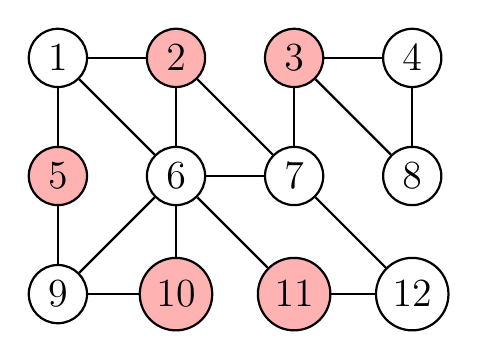
\begin{tikzpicture}[-,auto,node distance=1.5cm,
                    thick,main node/.style={circle,fill=white,draw,font=\sffamily\Large\bfseries}]

  \node[main node] (1) {$1$};
  \node[main node,fill=red!30] (2) [right of=1] {$2$};
  \node[main node,fill=red!30] (3) [right of=2]  {$3$};
  \node[main node] (4) [right of=3]  {$4$};
  \node[main node,fill=red!30] (5) [below of=1]  {$5$};
  \node[main node] (6) [below of=2]  {$6$};
  \node[main node] (7) [below of=3]  {$7$};
  \node[main node] (8) [below of=4]  {$8$};
  \node[main node] (9) [below of=5]  {$9$};
  \node[main node,fill=red!30] (10) [below of=6]  {$10$};
  \node[main node,fill=red!30] (11) [below of=7] {$11$};
  \node[main node] (12) [below of=8] {$12$}; 

  \path[every node/.style={font=\sffamily}]
    (1) edge (2)
    (1) edge (5)
    (1) edge (6)
    (2) edge (6)
    (2) edge (7)
    (3) edge (7)
    (3) edge (4)
    (3) edge (8)
    (4) edge (8)
    (5) edge (9)
    (6) edge (7)
    (6) edge (10)
    (6) edge (11)
    (6) edge (9)
    (7) edge (12)
    (9) edge (10)
    (11) edge (12)
    ;
\end{tikzpicture}}    
\end{center}
\caption{$2$-polygonal attack on $D=\{2,3,5,10,11  \}$ }
\end{figure}
Giving $V \leq \max\{\frac{1}{5},\frac{m}{10} \}$.
      \end{minipage}


    \end{columns}


\end{frame}

%
%\section[]{Introduction to the elongated star}
%\hypertarget{Introduction to the elongated star}{}
%\begin{frame}{\insertsection}
%
%
%We now wish to integrate features of a star into a line.
%We will form the elongated star $S_{n}^{k}$. We will use the labelling as below
%
%\begin{figure}
%\begin{center}
%\begin{tikzpicture}[-,auto,node distance=1.5cm,
%                    thick,main node/.style={circle,draw,font=\sffamily\Large\bfseries}]
%
%  \node[main node] (1) {$1$};
%  \node[main node] (2) [right of=1] {$2$};
%  \node[main node] (3) [right of=2] {$3$};
%  \node[main node] (4) [right of=3] {$4$};
%  \node[main node] (5) [right of=4] {$5$};
%  \node[main node] (6) [right of=5]  {$6$};
%  \node[main node] (7) [right of=6]  {$c$};
%  \node[main node] (8) [right of=7]  {$*$};
%  \node[main node] (9) [above of=7]  {$*$};
%  \node[main node] (10) [below of=7]  {$*$};
%  
%
%  \path[every node/.style={font=\sffamily}]
%    (1) edge  (2)
%    (2) edge (3)
%    (3) edge (4)
%    (4) edge (5)
%    (5) edge (6)
%    (6) edge (7)
%    (7) edge (8)
%     edge (9)
%     edge (10);
%\end{tikzpicture}
%\end{center}
%\caption{Labeling on the graph $S_{4}^5$.}
%\end{figure}
%
%\end{frame}
%
%\begin{frame}{\insertsection}
%
%\begin{definition}[Random Oscillation]
%The \textit{Oscillation} on $S_{n}^{k}$ is any embedded Hamiltonian Patrol on $C_{2(n+k)}$.
%
%The \textit{Random Oscillation} on $S_{n}^{k}$ is the embedded Random Hamiltonian Patrol on $C_{2(n+k)}$.
%\end{definition}
%
%\begin{figure}
%\begin{center}
%\resizebox{\textwidth}{!}{
%\begin{tikzpicture}[baseline=(current bounding box.north),-,auto,node distance=1cm,
%                    thick,main node/.style={circle,draw,font=\sffamily\bfseries}]
%
%  \node[main node] (1) {$3$};
%  \node[main node] (2) [above right of=1] {$4$};
%  \node[main node] (3) [right of=2] {$5$};
%  \node[main node] (4) [right of=3] {$6$};
%  \node[main node] (5) [right of=4] {$7$};
%  \node[main node] (6) [below right of=5] {$8$};
%  \node[main node] (7) [below right of=1] {$2$};
%  \node[main node] (8) [right of=7] {$1$};
%  \node[main node] (9) [right of=8] {$10$};
%  \node[main node] (10) [right of=9] {$9$};
%  
%  \node (P1) [right of=6] {};
%  \node (P2) [right of=P1] {};
%  
%  \node[main node] (a) [right of=P2] {$1$};
%  \node[main node] (b) [right of=a] {$2$};
%  \node[main node] (c) [right of=b] {$3$};
%  \node[main node] (d) [right of=c] {$c$};
%  \node[main node] (e) [right of=d] {$*$};
%  \node[main node] (f) [above of=d] {$*$};
%  
%  \draw[->] (P1) edge (P2);
%  
%
%  \path[every node/.style={font=\sffamily}]
%    (1) edge  (2)
%    edge (7)
%    (2) edge (3)
%    (3) edge (4)
%    (4) edge (5)
%    (5) edge (6)
%    (6) edge (10)
%    (7) edge (8)
%    (8) edge (9)
%    (9) edge (10)
%    (a) edge (b)
%    (b) edge (c)
%    (c) edge (d)
%    (d) edge (e)
%    edge (f);
%    
%     \path[dashed,red,every node/.style={font=\sffamily}]
%    (2) edge  (7)
%    (3) edge (8);
%    
%    \path[dashed,blue,every node/.style={font=\sffamily}]
%    (4) edge  (9);
%    
%    \path[dashed,blue,out=-60,in=180,every node/.style={font=\sffamily}]
%    (4) edge (6);
%    
%    \path[dashed,blue,out=60,in=180,every node/.style={font=\sffamily}]
%    (9) edge (6);
%  
%  \node (Box1) [draw,thick,fit=(1) (2) (3) (7) (8),fill,red,opacity=0.2] {};
%  \node (Box2) [draw,thick,fit=(4) (5) (6)  (10),fill,blue,opacity=0.2] {};
%  
%  \node (Box3) [draw,thick,fit=(a) (b) (c),fill,red,opacity=0.2] {}; 
%  \node (Box4) [draw,thick,fit=(d) (e) (f),fill,blue,opacity=0.2] {};   
%  
%\node [left=0.5cm,above=0.5cm,text width=0.5cm] at (2) {$C_{10}$};
%\node [left=0.5cm,above=0.5cm,text width=0.5cm] at (a) {$S_{3}^{2}$};   
%\end{tikzpicture}
%}
%\end{center}
%\caption{$C_{10}$ can be simplified to $S_{3}^{2}$ by node identifying.}
%\end{figure}
%
%\end{frame}
%
%\begin{frame}{\insertsection}
%
%\begin{lemma}
%For $m < 2(n+k)$ following the Random Oscillation,
%$$V(S_{n}^{k}) \geq V(C_{2(n+k)})=\frac{m}{2(n+k)}$$
%and if $m \geq 2(n+k)$ then $V(S_{n}^{k})=1$, achieved by any Oscillation.
%\end{lemma}
%
%This is again because the patroller can do no worse following the embedded path from $C_{2(n+k)}$ in $S_{n}^{k}$ 
%
%\end{frame}
%
%\begin{frame}{\insertsection}
%We adapt the time limited diametric attack to the time-delayed attack.
%
%\begin{definition}[Time-delayed attack]
%Let the \textit{time-delayed attack}, be the attack that attacks at the extended node labelled $1$ with probability $\frac{k+1}{n+k}$ and a particular normal node labelled $*$ with probability $\frac{1}{n+k}$.
%
%If node $1$ is chosen have the attack choose probability intervals with equal probability starting attacks at $\tau, \tau+1,...,\tau+2k+1$. If a $*$ node is chosen start the attacks at the times $\tau+k,\tau+k+1$ with equal probability.
%\end{definition}
%
%\begin{figure}
%\begin{center}
%\begin{tikzpicture}
% %Drawing Bottom Axis
% \draw[->] (-4,0) -- (4,0);
% \node (timelabel) [shift={(0.2,0)}] at (4,0) {$t$};
% \draw (-3.5,0.2) -- (-3.5,-0.2);
% \draw (3.5,0.2) -- (3.5,-0.2);
% 
% %Drawing Cross and lines 
% \node (labelc1) at (-3.5,-0.5) {$\tau$};
% \node (labelc2) at (3.5,-0.5) {$\tau+2k+1$};
% 
% \node[cross=5pt,red] (c1) at (-3.5,0.5) {};
% \node[cross=5pt,red] (c2) at (3.5,0.5) {};
% \draw[dashed] (c1) -- (c2);
% \node (linelabel1) at (-4.4,0.5) {Type $1$};
% 
% 
% \draw (-1,0.2) -- (-1,-0.2);
% \draw (1,0.2) -- (1,-0.2);
% 
%  \node (labelc3) at (-1,-0.5) {$\tau+k$};
% \node (labelc4) at (1,-0.5) {$\tau+k+1$};
% 
% \node[cross=5pt,red] (c3) at (-1,1) {};
% \node[cross=5pt,red] (c4) at (1,1) {};
% \draw[dashed] (c3) -- (c4);
% \node (linelabel1) at (-1.9,1) {Type $*$}; 
%
%\end{tikzpicture}
%\end{center}
%\end{figure}
%
%
%
%\end{frame}
%
%\begin{frame}{\insertsection}
%
%\begin{lemma}
%When $T \geq m+2k$, the upper bound $V \leq \max \left\{ \frac{k+1}{n+k} , \frac{m}{2(n+k)}   \right\}$
%\end{lemma}
%
%Hence we have a partial solution, analogous to \textcolor{yellow}{region 1} and \textcolor{red}{region 2} for the line.
%
%\begin{theorem}
%If $T \geq m+2k$ and $ m \geq 2(k+1)$ then we have the value of the game is
%
%\begin{equation}
%V=\min \left\{1,\frac{m}{2(n+k)} \right\} 
%\end{equation}
%\end{theorem}
%
%\end{frame}
%
%\begin{frame}{\insertsection}
%
%\begin{figure}
%\resizebox{0.95\linewidth}{!}{
%% Created by tikzDevice version 0.10.1 on 2017-11-10 10:35:56
% !TEX encoding = UTF-8 Unicode
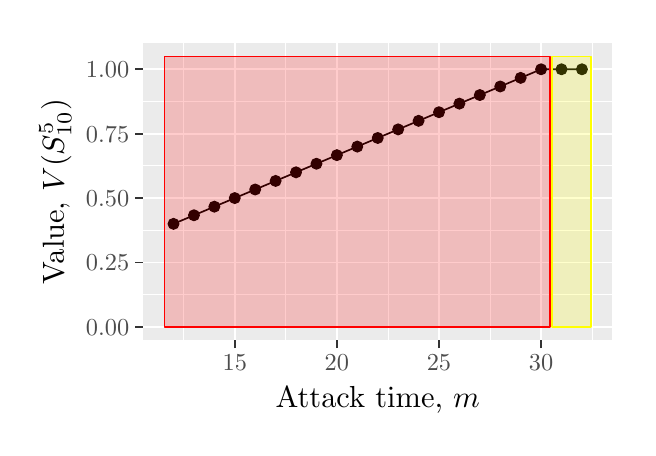
\begin{tikzpicture}[x=1pt,y=1pt]
\definecolor{fillColor}{RGB}{255,255,255}
\path[use as bounding box,fill=fillColor,fill opacity=0.00] (0,0) rectangle (216.81,144.54);
\begin{scope}
\path[clip] (  0.00,  0.00) rectangle (216.81,144.54);
\definecolor{drawColor}{RGB}{255,255,255}
\definecolor{fillColor}{RGB}{255,255,255}

\path[draw=drawColor,line width= 0.6pt,line join=round,line cap=round,fill=fillColor] (  0.00,  0.00) rectangle (216.81,144.54);
\end{scope}
\begin{scope}
\path[clip] ( 41.67, 31.53) rectangle (211.31,139.04);
\definecolor{fillColor}{gray}{0.92}

\path[fill=fillColor] ( 41.67, 31.53) rectangle (211.31,139.04);
\definecolor{drawColor}{RGB}{255,255,255}

\path[draw=drawColor,line width= 0.3pt,line join=round] ( 41.67, 48.05) --
	(211.31, 48.05);

\path[draw=drawColor,line width= 0.3pt,line join=round] ( 41.67, 71.32) --
	(211.31, 71.32);

\path[draw=drawColor,line width= 0.3pt,line join=round] ( 41.67, 94.59) --
	(211.31, 94.59);

\path[draw=drawColor,line width= 0.3pt,line join=round] ( 41.67,117.86) --
	(211.31,117.86);

\path[draw=drawColor,line width= 0.3pt,line join=round] ( 56.39, 31.53) --
	( 56.39,139.04);

\path[draw=drawColor,line width= 0.3pt,line join=round] ( 93.28, 31.53) --
	( 93.28,139.04);

\path[draw=drawColor,line width= 0.3pt,line join=round] (130.18, 31.53) --
	(130.18,139.04);

\path[draw=drawColor,line width= 0.3pt,line join=round] (167.07, 31.53) --
	(167.07,139.04);

\path[draw=drawColor,line width= 0.3pt,line join=round] (203.97, 31.53) --
	(203.97,139.04);

\path[draw=drawColor,line width= 0.6pt,line join=round] ( 41.67, 36.42) --
	(211.31, 36.42);

\path[draw=drawColor,line width= 0.6pt,line join=round] ( 41.67, 59.69) --
	(211.31, 59.69);

\path[draw=drawColor,line width= 0.6pt,line join=round] ( 41.67, 82.96) --
	(211.31, 82.96);

\path[draw=drawColor,line width= 0.6pt,line join=round] ( 41.67,106.23) --
	(211.31,106.23);

\path[draw=drawColor,line width= 0.6pt,line join=round] ( 41.67,129.50) --
	(211.31,129.50);

\path[draw=drawColor,line width= 0.6pt,line join=round] ( 74.83, 31.53) --
	( 74.83,139.04);

\path[draw=drawColor,line width= 0.6pt,line join=round] (111.73, 31.53) --
	(111.73,139.04);

\path[draw=drawColor,line width= 0.6pt,line join=round] (148.63, 31.53) --
	(148.63,139.04);

\path[draw=drawColor,line width= 0.6pt,line join=round] (185.52, 31.53) --
	(185.52,139.04);
\definecolor{drawColor}{RGB}{0,0,0}
\definecolor{fillColor}{RGB}{0,0,0}

\path[draw=drawColor,line width= 0.4pt,line join=round,line cap=round,fill=fillColor] (192.90,129.50) circle (  1.96);

\path[draw=drawColor,line width= 0.4pt,line join=round,line cap=round,fill=fillColor] (200.28,129.50) circle (  1.96);

\path[draw=drawColor,line width= 0.4pt,line join=round,line cap=round,fill=fillColor] ( 52.70, 73.65) circle (  1.96);

\path[draw=drawColor,line width= 0.4pt,line join=round,line cap=round,fill=fillColor] ( 60.08, 76.75) circle (  1.96);

\path[draw=drawColor,line width= 0.4pt,line join=round,line cap=round,fill=fillColor] ( 67.46, 79.86) circle (  1.96);

\path[draw=drawColor,line width= 0.4pt,line join=round,line cap=round,fill=fillColor] ( 74.83, 82.96) circle (  1.96);

\path[draw=drawColor,line width= 0.4pt,line join=round,line cap=round,fill=fillColor] ( 82.21, 86.06) circle (  1.96);

\path[draw=drawColor,line width= 0.4pt,line join=round,line cap=round,fill=fillColor] ( 89.59, 89.16) circle (  1.96);

\path[draw=drawColor,line width= 0.4pt,line join=round,line cap=round,fill=fillColor] ( 96.97, 92.27) circle (  1.96);

\path[draw=drawColor,line width= 0.4pt,line join=round,line cap=round,fill=fillColor] (104.35, 95.37) circle (  1.96);

\path[draw=drawColor,line width= 0.4pt,line join=round,line cap=round,fill=fillColor] (111.73, 98.47) circle (  1.96);

\path[draw=drawColor,line width= 0.4pt,line join=round,line cap=round,fill=fillColor] (119.11,101.57) circle (  1.96);

\path[draw=drawColor,line width= 0.4pt,line join=round,line cap=round,fill=fillColor] (126.49,104.68) circle (  1.96);

\path[draw=drawColor,line width= 0.4pt,line join=round,line cap=round,fill=fillColor] (133.87,107.78) circle (  1.96);

\path[draw=drawColor,line width= 0.4pt,line join=round,line cap=round,fill=fillColor] (141.25,110.88) circle (  1.96);

\path[draw=drawColor,line width= 0.4pt,line join=round,line cap=round,fill=fillColor] (148.63,113.99) circle (  1.96);

\path[draw=drawColor,line width= 0.4pt,line join=round,line cap=round,fill=fillColor] (156.00,117.09) circle (  1.96);

\path[draw=drawColor,line width= 0.4pt,line join=round,line cap=round,fill=fillColor] (163.38,120.19) circle (  1.96);

\path[draw=drawColor,line width= 0.4pt,line join=round,line cap=round,fill=fillColor] (170.76,123.29) circle (  1.96);

\path[draw=drawColor,line width= 0.4pt,line join=round,line cap=round,fill=fillColor] (178.14,126.40) circle (  1.96);

\path[draw=drawColor,line width= 0.4pt,line join=round,line cap=round,fill=fillColor] (185.52,129.50) circle (  1.96);

\path[draw=drawColor,line width= 0.6pt,line join=round] ( 52.70, 73.65) --
	( 60.08, 76.75) --
	( 67.46, 79.86) --
	( 74.83, 82.96) --
	( 82.21, 86.06) --
	( 89.59, 89.16) --
	( 96.97, 92.27) --
	(104.35, 95.37) --
	(111.73, 98.47) --
	(119.11,101.57) --
	(126.49,104.68) --
	(133.87,107.78) --
	(141.25,110.88) --
	(148.63,113.99) --
	(156.00,117.09) --
	(163.38,120.19) --
	(170.76,123.29) --
	(178.14,126.40) --
	(185.52,129.50) --
	(192.90,129.50) --
	(200.28,129.50);
\definecolor{drawColor}{RGB}{255,255,0}
\definecolor{fillColor}{RGB}{255,255,0}

\path[draw=drawColor,line width= 0.6pt,line join=round,fill=fillColor,fill opacity=0.20] (189.58, 36.42) rectangle (203.60,134.15);
\definecolor{drawColor}{RGB}{255,0,0}
\definecolor{fillColor}{RGB}{255,0,0}

\path[draw=drawColor,line width= 0.6pt,line join=round,fill=fillColor,fill opacity=0.20] ( 49.38, 36.42) rectangle (188.84,134.15);
\end{scope}
\begin{scope}
\path[clip] (  0.00,  0.00) rectangle (216.81,144.54);
\definecolor{drawColor}{gray}{0.30}

\node[text=drawColor,anchor=base east,inner sep=0pt, outer sep=0pt, scale=  0.88] at ( 36.72, 33.39) {0.00};

\node[text=drawColor,anchor=base east,inner sep=0pt, outer sep=0pt, scale=  0.88] at ( 36.72, 56.66) {0.25};

\node[text=drawColor,anchor=base east,inner sep=0pt, outer sep=0pt, scale=  0.88] at ( 36.72, 79.93) {0.50};

\node[text=drawColor,anchor=base east,inner sep=0pt, outer sep=0pt, scale=  0.88] at ( 36.72,103.20) {0.75};

\node[text=drawColor,anchor=base east,inner sep=0pt, outer sep=0pt, scale=  0.88] at ( 36.72,126.47) {1.00};
\end{scope}
\begin{scope}
\path[clip] (  0.00,  0.00) rectangle (216.81,144.54);
\definecolor{drawColor}{gray}{0.20}

\path[draw=drawColor,line width= 0.6pt,line join=round] ( 38.92, 36.42) --
	( 41.67, 36.42);

\path[draw=drawColor,line width= 0.6pt,line join=round] ( 38.92, 59.69) --
	( 41.67, 59.69);

\path[draw=drawColor,line width= 0.6pt,line join=round] ( 38.92, 82.96) --
	( 41.67, 82.96);

\path[draw=drawColor,line width= 0.6pt,line join=round] ( 38.92,106.23) --
	( 41.67,106.23);

\path[draw=drawColor,line width= 0.6pt,line join=round] ( 38.92,129.50) --
	( 41.67,129.50);
\end{scope}
\begin{scope}
\path[clip] (  0.00,  0.00) rectangle (216.81,144.54);
\definecolor{drawColor}{gray}{0.20}

\path[draw=drawColor,line width= 0.6pt,line join=round] ( 74.83, 28.78) --
	( 74.83, 31.53);

\path[draw=drawColor,line width= 0.6pt,line join=round] (111.73, 28.78) --
	(111.73, 31.53);

\path[draw=drawColor,line width= 0.6pt,line join=round] (148.63, 28.78) --
	(148.63, 31.53);

\path[draw=drawColor,line width= 0.6pt,line join=round] (185.52, 28.78) --
	(185.52, 31.53);
\end{scope}
\begin{scope}
\path[clip] (  0.00,  0.00) rectangle (216.81,144.54);
\definecolor{drawColor}{gray}{0.30}

\node[text=drawColor,anchor=base,inner sep=0pt, outer sep=0pt, scale=  0.88] at ( 74.83, 20.52) {15};

\node[text=drawColor,anchor=base,inner sep=0pt, outer sep=0pt, scale=  0.88] at (111.73, 20.52) {20};

\node[text=drawColor,anchor=base,inner sep=0pt, outer sep=0pt, scale=  0.88] at (148.63, 20.52) {25};

\node[text=drawColor,anchor=base,inner sep=0pt, outer sep=0pt, scale=  0.88] at (185.52, 20.52) {30};
\end{scope}
\begin{scope}
\path[clip] (  0.00,  0.00) rectangle (216.81,144.54);
\definecolor{drawColor}{RGB}{0,0,0}

\node[text=drawColor,anchor=base,inner sep=0pt, outer sep=0pt, scale=  1.10] at (126.49,  7.44) {Attack time, $m$};
\end{scope}
\begin{scope}
\path[clip] (  0.00,  0.00) rectangle (216.81,144.54);
\definecolor{drawColor}{RGB}{0,0,0}

\node[text=drawColor,rotate= 90.00,anchor=base,inner sep=0pt, outer sep=0pt, scale=  1.10] at ( 13.08, 85.29) {Value, $V(S_{ 10 }^{ 5 })$};
\end{scope}
\end{tikzpicture}
}
%\caption{Value of the Star Graph, $S_{10}^{5}$}
%\end{figure}
%
%
%\end{frame}

\section[]{Future Work}
\hypertarget{Future work}{}
\begin{frame}{\insertsection}

\begin{itemize}
\item Look at analysing different types of Polygonal attacks, i.e the best choice of $d$ and how to select the set $D$.
\item Look at analysing the elongated star graph, that is the star graph with one of the end points further away from the centre.
\item Alter the problem to have `semi-random' attackers arriving on predetermined sections of the graph.
\end{itemize}

\end{frame}



\begin{frame}[plain,noframenumbering]{Nash equilibria and optimal solutions}
\begin{definition}[Mixed Nash equilibrium]
A choice of $\bm{\pi}^*$ and $\bm{\phi}^*$ is said to be in \textit{Nash equilibrium} if 
\begin{align*}
P(\bm{\pi}^*,\bm{\phi}^*) \geq P(\bm{\pi},\bm{\phi}^*) \quad \forall \bm{\pi} \in \Pi , \\
P(\bm{\pi}^*,\bm{\phi}^*) \geq P(\bm{\pi}^*,\bm{\phi}) \quad \forall \bm{\phi} \in \Phi .
\end{align*}
\end{definition}

\pause

\begin{definition}[Optimal solution]
let $N$ be the set of all Nash equilibria then we say that $(\bm{\pi}^{*},\bm{\phi}^{*}) \in N$ is an \textit{optimal solution} if
$$P(\bm{\pi}^{*},\bm{\phi}^{*}) \geq P(n) \quad \forall n \in N$$ 
\end{definition}

\textbf{Note.} It is possible that no optimal solution exists

\pause

Luckily in zero-sum games are guaranteed to to have at least one optimal solution and any nash-equilbrium is optimal.

\end{frame}

\begin{frame}[plain,noframenumbering]{Game Value}

\begin{theorem}[Minimax Theorem (John Neumann, 1928)]
Let $X \subset \mathbb{R}^{n}$ and $Y \subset \mathbb{R}^{m}$ be compact convex sets and let $f: X \times Y \rightarrow \mathbb{R}$ be a continuous convex-concave function then
$$\min\limits_{x \in X} \max\limits_{y \in Y} f(x,y) = \max\limits_{y \in Y} \min\limits_{x \in X} f(x,y) $$
\end{theorem}

\textbf{Note.} Convex-concave means convex for a fixed $y$ and concave for a fixed $x$.

\pause
Now $\Pi$ and $\Phi$ are both compact convex sets and as our game is zero-sum our payoff function $P(\bm{\pi},\bm{\phi})$ is convex-concave. Solving the minimax problem is equivalent to Nash-equilibrium and are hence optimal solutions.


This gives rise to the game's value, as given by \textcolor{purple}{$$V(G) \equiv \max\limits_{\bm{\pi} \in \Pi} \min\limits_{\bm{\phi} \in \Phi} P(\bm{\pi},\bm{\phi})=\min\limits_{\bm{\phi} \in \Phi} \max\limits_{\bm{\pi} \in \Pi} P(\bm{\pi},\bm{\phi})$$}
\end{frame}


\end{document}
